\documentclass[11pt,a4paper]{article}
\usepackage[T1]{fontenc}\usepackage{lmodern}
\usepackage[a4paper,margin=23mm,includeheadfoot,headheight=15pt,headsep=15pt,footskip=22pt]{geometry}
\usepackage[nopatch=footnote]{microtype}
\usepackage{amsmath,amssymb,amsthm,mathtools,aliascnt}
\usepackage{booktabs,longtable,array,tabularx,enumitem,fancyhdr,graphicx}
\usepackage[table]{xcolor}\usepackage{setspace,needspace,listings,caption,titlesec,etoolbox}
\PassOptionsToPackage{hyphens}{url}\usepackage{hyperref}\usepackage[nameinlink,noabbrev]{cleveref}\usepackage{bookmark}
\definecolor{accent}{HTML}{137668}\definecolor{muted}{HTML}{536568}
\frenchspacing\emergencystretch=3em\clubpenalty=10000\widowpenalty=10000\raggedbottom
\titleformat{\section}{\sffamily\bfseries\large\color{accent}}{\thesection}{.7em}{}
\titleformat{\subsection}{\sffamily\bfseries\normalsize}{\thesubsection}{.7em}{}
\titlespacing*{\section}{0pt}{1.4\baselineskip}{.55\baselineskip}
\captionsetup{font=small,labelfont={sf,bf},labelsep=period}
\pretocmd{\section}{\Needspace{7\baselineskip}}{}{}\pretocmd{\subsection}{\Needspace{5\baselineskip}}{}{}
\allowdisplaybreaks\setstretch{1.055}\setlength{\parskip}{.3em}\setlength{\parindent}{1.35em}
\setlist[itemize]{topsep=.35em,itemsep=.15em,leftmargin=1.6em}\setlist[enumerate]{topsep=.35em,itemsep=.15em,leftmargin=1.8em}
\graphicspath{{figures/}}
\hypersetup{pdftitle={Projector-Resolved Seed Calculus II: Refinement, Weighted Transfer and Integral Separation},pdfauthor={Komorebi P.},colorlinks=true,linkcolor=accent,citecolor=accent,urlcolor=accent}
\pagestyle{fancy}\fancyhf{}
\fancyhead[L]{\sffamily\fontsize{8}{10}\selectfont\color{muted}KOMOREBI MATHEMATICS / PAPER II}
\fancyhead[R]{\sffamily\fontsize{8}{10}\selectfont\color{muted}TRADITIONAL PAPER}
\fancyfoot[L]{\sffamily\fontsize{8}{10}\selectfont\color{muted}Projector-resolved seed calculus}\fancyfoot[R]{\sffamily\small\color{accent}\thepage}
\lstset{basicstyle=\ttfamily\footnotesize,breaklines=true,frame=single,showstringspaces=false,columns=fullflexible,keepspaces=true}
\newtheorem{theorem}{Theorem}[section]
\newaliascnt{proposition}{theorem}
\newtheorem{proposition}[proposition]{Proposition}
\aliascntresetthe{proposition}
\newaliascnt{lemma}{theorem}
\newtheorem{lemma}[lemma]{Lemma}
\aliascntresetthe{lemma}
\newaliascnt{corollary}{theorem}
\newtheorem{corollary}[corollary]{Corollary}
\aliascntresetthe{corollary}
\theoremstyle{definition}
\newaliascnt{definition}{theorem}
\newtheorem{definition}[definition]{Definition}
\aliascntresetthe{definition}
\newaliascnt{example}{theorem}
\newtheorem{example}[example]{Example}
\aliascntresetthe{example}
\newaliascnt{standardfact}{theorem}
\newtheorem{standardfact}[standardfact]{Standard Fact}
\aliascntresetthe{standardfact}
\theoremstyle{remark}
\newaliascnt{remark}{theorem}
\newtheorem{remark}[remark]{Remark}
\aliascntresetthe{remark}

\crefname{theorem}{theorem}{theorems}
\crefname{proposition}{proposition}{propositions}
\crefname{lemma}{lemma}{lemmas}
\crefname{corollary}{corollary}{corollaries}
\crefname{definition}{definition}{definitions}
\crefname{example}{example}{examples}
\crefname{standardfact}{standard fact}{standard facts}
\crefname{remark}{remark}{remarks}

\newcommand{\bbk}{\Bbbk}
\newcommand{\OO}{\mathcal O}
\newcommand{\Acal}{\mathcal A}
\newcommand{\Bcal}{\mathcal B}
\newcommand{\Pcal}{\mathcal P}
\newcommand{\Qcal}{\mathcal Q}
\newcommand{\Scal}{\mathcal S}
\newcommand{\Rcal}{\mathcal R}
\newcommand{\End}{\operatorname{End}}
\newcommand{\im}{\operatorname{im}}
\newcommand{\Ker}{\operatorname{Ker}}
\newcommand{\coker}{\operatorname{coker}}
\newcommand{\Frac}{\operatorname{Frac}}
\newcommand{\length}{\operatorname{length}}
\newcommand{\val}{\operatorname{val}}
\newcommand{\wt}{\operatorname{wt}}
\newcommand{\Supp}{\operatorname{Supp}}
\newcommand{\id}{\mathrm{id}}
\newcommand{\diag}{\operatorname{diag}}
\newcommand{\Res}{\operatorname{Res}}
\newcommand{\lcmop}{\operatorname{lcm}}
\newcommand{\expn}{\operatorname{exp}}

\providecommand{\Seed}{\mathfrak S}
\providecommand{\cX}{\mathcal X}
\providecommand{\cA}{\mathcal A}
\providecommand{\cB}{\mathcal B}
\providecommand{\cC}{\mathcal C}
\providecommand{\cD}{\mathcal D}
\providecommand{\cF}{\mathcal F}
\providecommand{\cG}{\mathcal G}
\providecommand{\cO}{\mathcal O}
\providecommand{\cP}{\mathcal P}
\providecommand{\cR}{\mathcal R}
\providecommand{\cS}{\mathcal S}
\providecommand{\cT}{\mathcal T}
\providecommand{\End}{\operatorname{End}}
\providecommand{\Hom}{\operatorname{Hom}}
\providecommand{\im}{\operatorname{im}}
\providecommand{\Ker}{\operatorname{Ker}}
\providecommand{\Spec}{\operatorname{Spec}}
\providecommand{\Res}{\operatorname{Res}}
\providecommand{\Hol}{\operatorname{Hol}}
\providecommand{\Tr}{\operatorname{Tr}}
\providecommand{\diag}{\operatorname{diag}}
\providecommand{\id}{\mathrm{id}}
\providecommand{\bbk}{\mathbb{k}}
\providecommand{\N}{\mathbb N}
\providecommand{\Z}{\mathbb Z}
\providecommand{\C}{\mathbb C}
\providecommand{\Q}{\mathbb Q}
\providecommand{\F}{\mathbb F}
\providecommand{\OO}{\mathcal O}
\providecommand{\Frac}{\operatorname{Frac}}
\providecommand{\val}{\operatorname{val}}
\providecommand{\wt}{\operatorname{wt}}
\providecommand{\lcm}{\operatorname{lcm}}
\providecommand{\packet}[2]{#1_{#2}}
\newcolumntype{L}[1]{>{\raggedright\arraybackslash}p{#1}}
\newcolumntype{Y}{>{\raggedright\arraybackslash}X}


\theoremstyle{definition}\newtheorem{construction}[theorem]{Construction}\newtheorem{certificate}[theorem]{Numerical Certificate}
\theoremstyle{remark}\newtheorem{boundary}[theorem]{Boundary}

% Operation Komorebi: shared publication profile.
\usepackage{komorebi-publication}
\renewcommand{\KomorebiTitle}{Projector-Resolved Seed Calculus II}
\renewcommand{\KomorebiSubtitle}{Refinement towers, weighted transfer, and integral separation of operator packets}
\renewcommand{\KomorebiSeries}{Core series II}
\renewcommand{\KomorebiKind}{Traditional paper}
\renewcommand{\KomorebiEdition}{Standardized publication edition / 8 October 2026}
\renewcommand{\KomorebiShortTitle}{Paper II}
\renewcommand{\KomorebiTitleSize}{31}
\renewcommand{\KomorebiTitleLeading}{36}
\renewcommand{\KomorebiProfile}{classical}
\renewcommand{\KomorebiOrientation}{portrait}
\KomorebiSetup
\begin{document}
\KomorebiCover
\KomorebiOpeningNote{\textbf{Reading route.} Exact coordinates and residue selectors lead to weighted inversion and rational walk series.  Integral lattice gluing then gives exact separation weights and precision delays.  Smith congruences and typed defect formulas connect the algebra to finite computation and operator calculus.

\medskip
\textbf{Scope.} Full ordinary proofs and the revised 25-row formal contract are distinguished throughout.  The expanded analytic and lattice results retain their own hypotheses; inherited formal coverage does not expand merely because both presentations appear in this edition.}


\begin{abstract}

A complete family of idempotents gives exact coordinates, but a single family does not record scale or integral visibility.  We study towers in which every coarse idempotent is the sum of its fine descendants.  The coordinate changes are invertible and coherent, and every operator block is the sum of its refined blocks.  Residue selectors give a model over arbitrary rings.  When roots of unity are available they agree with character averages, and coprime moduli factor through the Chinese remainder theorem.  In a complete filtered algebra, a diagonal operator plus positive weight transfers has an inverse obtained by summing admissible weighted paths.  The formula truncates exactly at finite precision, while finite transfer graphs have rational path series.  For a rational spectral decomposition over a discrete valuation ring, resultants give denominator bounds.  The exact denominator is the largest Smith exponent of the lattice gluing module.  This yields a necessary and sufficient precision delay, monotonicity under refinement, and a full congruence solving formula.  We close with exact formulas for the propagation of a coarse graining defect through powers, resolvents, holomorphic functions, exponentials, and multilevel towers.
\end{abstract}
\noindent This edition integrates the expanded mathematical narrative with the canonical v1.2.1 certificate-level formulations.  It preserves the distinction between general written proofs, formal specifications, and finite computational examples.  A separate visual guide and a Lean guide provide worked models and the complete formal-contract crosswalk.
\tableofcontents\listoffigures\listoftables\clearpage
\section{Introduction}

A complete family of pairwise annihilating idempotents decomposes a module into exact coordinate pieces.  Many problems require more than one such decomposition.  A signal may be split first into two residue classes and then into four.  A filtered operator may be resolved into transfers that appear at different valuation depths.  A rational spectral splitting may exist over the fraction field while remaining invisible on the original lattice.  These are all refinement problems, but they involve different notions of scale.

The first part of the article concerns exact refinement.  If a fine packet family refines a coarse family, then each coarse idempotent is the sum of its fine descendants.  The coordinate spaces at the two levels are canonically isomorphic because both represent the whole module.  The refinement relation adds more information.  It tells us which fine coordinates belong to each coarse coordinate, and it gives a compatible decomposition of every operator block.  This is the algebra behind polyphase coordinates and nested filter banks.  Standard treatments of those subjects may be found in \cite{Vaidyanathan1993,Daubechies1992}.

The second part studies inversion in a complete filtered algebra.  Suppose an operator has the form
\[
T=D+N,
\]
where $D$ is invertible and every packet transfer in $N$ raises the filtration by a positive amount.  The ordinary Neumann series can then be expanded into weighted paths.  The weight is not the number of edges.  It is the total filtration gain along the path.  At precision $L$, every path of weight at least $L$ vanishes.  A finite transfer graph also gives a rational generating function for the number of paths of each total weight.  The relevant generating function facts are classical and are discussed in \cite{Stanley2012}.

The third part concerns integral separation.  Let $V$ be a vector space over the fraction field of a discrete valuation ring $\OO$, and let $\Lambda$ be an $\OO$ lattice in $V$.  A rational projector $E$ need not preserve $\Lambda$.  Its separation weight is the least $s$ such that
\[
\pi^sE\Lambda\subseteq\Lambda.
\]
A Bézout construction gives an upper bound through a polynomial resultant.  That bound need not be exact because it does not see the position of the lattice.  The exact answer is controlled by the finite module
\[
G_{\Lambda,\Pcal}
=
\Lambda\Big/\bigoplus_{\alpha}(\Lambda\cap V_\alpha),
\]
where $V=\bigoplus_\alpha V_\alpha$ is the rational packet decomposition.  The largest Smith exponent of this gluing module is exactly the common denominator needed to make every packet projector integral.  This interpretation also proves that separation weight cannot decrease under refinement.  Background on local fields, Smith normal form, and matrix polynomials may be found in \cite{Serre1979,Newman1972,GohbergLancasterRodman2009}.

The last part records how a defect between fine and coarse operators propagates.  If
\[
\Delta=CT_f-T_cC,
\]
then exact formulas describe the corresponding defect for powers, resolvents, holomorphic functions, exponentials, and a chain of several refinement levels.  These formulas are elementary, but collecting them in one place makes the later analytic uses transparent.  The spectral and resolvent background follows the usual operator theory in \cite{Kato1995}.

The paper remains linear.  Exact refinement is not approximation, and no packet is discarded.  Nonlinear operation trees, nonlinear correction, and obstruction complexes require a separate theory.

\section{Four kinds of depth}\label{sec:four_depths}

Several quantities below are measured by nonnegative integers.  They do not measure the same thing.  Keeping them separate makes the later formulas easier to read.

The first is packet depth.  A finer packet family has more idempotents and a more detailed address set.  The passage from residues modulo two to residues modulo four is an example.  Packet depth is combinatorial.  It says how many distinctions have been made in the coordinate system.

The second is filtration depth.  A transfer in $F^r\Bcal$ is invisible modulo $F^r\Bcal$ and becomes visible at greater precision.  Two paths with the same number of edges can have different filtration depths.  A longer path can appear earlier when its edges have smaller weights.

The third is separation depth.  A rational packet projector may require multiplication by $\pi^s$ before it preserves the chosen lattice.  This number depends on both the rational decomposition and the lattice.  It can be zero even when the corresponding eigenvalues are close, and it can be positive even when the rational projector is simple.

The fourth is compatibility depth.  A fine operator and a separately chosen coarse operator need not commute with coarsening.  Their discrepancy is
\[
\Delta=CT_f-T_cC.
\]
This is not a packet depth or a denominator.  It measures the failure of one operator model to represent another exactly.

The four notions meet in applications, but no one of them determines the others.  An exact refinement tower may have zero coordinate error while its fine spectral packets have positive lattice weight.  A filtered inverse may truncate exactly at a given depth while the coarse operator still has a nonzero compatibility defect.  The paper treats each quantity with its own theorem before combining them.

A simple two packet model already contains all four ideas.  Let
\[
X=X_0\oplus X_1,
\qquad
D=\begin{pmatrix}D_0&0\\0&D_1\end{pmatrix},
\qquad
N=\begin{pmatrix}0&N_{01}\\N_{10}&0\end{pmatrix}.
\]
A finer family may split $X_0$ and $X_1$ into smaller summands.  The blocks $N_{01}$ and $N_{10}$ may enter at different filtration weights.  Over a fraction field, the rational packet spaces may fail to split the chosen lattice.  A coarse operator on one selected summand may also fail to intertwine with the full matrix.  The later sections isolate these four effects one at a time.

\section{Packet systems and refinement towers}\label{sec:refinement}

We begin with finite packet systems.  No inner product is needed.

\begin{definition}[Packet system]\label{def:packet_system}
Let $X$ be a module over a unital ring.  A finite packet system on $X$ is a family
\[
\Pcal=(P_\alpha)_{\alpha\in I}
\subseteq\End(X)
\]
of nonzero idempotents such that
\[
P_\alpha P_\beta=0
\quad\text{when }\alpha\ne\beta,
\qquad
\sum_{\alpha\in I}P_\alpha=I_X.
\]
Write
\[
X_\alpha=P_\alpha X,
\qquad
X^{\Pcal}=\bigoplus_{\alpha\in I}X_\alpha.
\]
The analysis and synthesis maps are
\[
\Acal_{\Pcal}x=(P_\alpha x)_\alpha,
\qquad
\Scal_{\Pcal}(x_\alpha)_\alpha=\sum_\alpha x_\alpha.
\]
They are inverse isomorphisms.
\end{definition}

\begin{definition}[Refinement]\label{def:refinement}\label{def:refinement-map}
Let $\Pcal=(P_\alpha)_{\alpha\in I}$ and $\Qcal=(Q_\beta)_{\beta\in J}$ be packet systems on the same module.  We say that $\Qcal$ refines $\Pcal$ when there is a surjection
\[
\rho:J\longrightarrow I
\]
such that
\[
P_\alpha=\sum_{\rho(\beta)=\alpha}Q_\beta
\]
for every $\alpha\in I$.  The index $\beta$ is then called a child of $\rho(\beta)$.
\end{definition}

\begin{theorem}[Children, parents, and transitivity]\label{thm:children_transitivity}\label{thm:nested-refinement}
Suppose that $\Qcal$ refines $\Pcal$ through $\rho$.  Then
\[
P_\alpha Q_\beta
=
Q_\beta P_\alpha
=
\begin{cases}
Q_\beta & \rho(\beta)=\alpha,\\
0 & \rho(\beta)\ne\alpha.
\end{cases}
\]
Hence $Q_\beta X\subseteq P_{\rho(\beta)}X$.  If a third packet system $\Rcal$ refines $\Qcal$, then $\Rcal$ refines $\Pcal$ through the composite parent map.
\end{theorem}

\begin{proof}
Multiply the identity
\[
P_\alpha=\sum_{\rho(\gamma)=\alpha}Q_\gamma
\]
by $Q_\beta$ on either side.  Pairwise annihilation in the fine family leaves $Q_\beta$ when $\rho(\beta)=\alpha$ and leaves zero otherwise.  For transitivity, substitute the child expansion of each $Q_\beta$ into the expansion of $P_\alpha$ and group the resulting terms by the composite parent.
\end{proof}

A refinement tower is a sequence $(\Pcal_\ell)_{\ell\geq0}$ with parent maps
\[
\rho_{m,\ell}:I_m\longrightarrow I_\ell
\qquad(m\geq\ell)
\]
that compose as expected.  The next result shows that the coordinate changes form a coherent system.

\begin{definition}[Coordinate change across levels]\label{def:coordinate_change}\label{def:coordinate-refinement}
For two packet systems $\Pcal$ and $\Qcal$ on $X$, define
\[
J_{\Qcal\leftarrow\Pcal}
=
\Acal_{\Qcal}\Scal_{\Pcal}:X^{\Pcal}\longrightarrow X^{\Qcal}
\]
and
\[
C_{\Pcal\leftarrow\Qcal}
=
\Acal_{\Pcal}\Scal_{\Qcal}:X^{\Qcal}\longrightarrow X^{\Pcal}.
\]
When $\Qcal$ refines $\Pcal$, the first map resolves each coarse coordinate into its children and the second adds the children back to their parent.
\end{definition}

\begin{theorem}[Exact coordinate change and coherence]\label{thm:coordinate_coherence}\label{prop:perfect-reconstruction}
For any two packet systems on $X$,
\[
C_{\Pcal\leftarrow\Qcal}J_{\Qcal\leftarrow\Pcal}=I_{X^{\Pcal}},
\qquad
J_{\Qcal\leftarrow\Pcal}C_{\Pcal\leftarrow\Qcal}=I_{X^{\Qcal}}.
\]
For three packet systems $\Pcal$, $\Qcal$, and $\Rcal$ on $X$,
\[
J_{\Rcal\leftarrow\Qcal}J_{\Qcal\leftarrow\Pcal}
=
J_{\Rcal\leftarrow\Pcal},
\]
\[
C_{\Pcal\leftarrow\Qcal}C_{\Qcal\leftarrow\Rcal}
=
C_{\Pcal\leftarrow\Rcal}.
\]
If $\Qcal$ refines $\Pcal$ through $\rho$, then
\[
\bigl(J_{\Qcal\leftarrow\Pcal}x\bigr)_\beta
=
Q_\beta x_{\rho(\beta)},
\qquad
\bigl(C_{\Pcal\leftarrow\Qcal}y\bigr)_\alpha
=
\sum_{\rho(\beta)=\alpha}y_\beta.
\]
\end{theorem}

\begin{proof}
The packet analysis and synthesis maps are inverse.  Therefore
\[
C_{\Pcal\leftarrow\Qcal}J_{\Qcal\leftarrow\Pcal}
=
\Acal_{\Pcal}\Scal_{\Qcal}\Acal_{\Qcal}\Scal_{\Pcal}
=
\Acal_{\Pcal}\Scal_{\Pcal}
=
I.
\]
The other inverse identity is the same calculation with the two systems exchanged.  The coherence identities follow by inserting
\[
\Scal_{\Qcal}\Acal_{\Qcal}=I_X.
\]
Now assume that $\Qcal$ refines $\Pcal$.  If $x=(x_\alpha)_\alpha$ with $x_\alpha\in P_\alpha X$, then
\[
Q_\beta\sum_\alpha x_\alpha
=
Q_\beta x_{\rho(\beta)}
\]
by \cref{thm:children_transitivity}.  The formula for $C$ follows by synthesis followed by projection onto the parent packet.
\end{proof}

\begin{remark}[Refinement and reduction]\label{rem:refinement_reduction}
The maps in \cref{thm:coordinate_coherence} are isomorphisms because both coordinate spaces represent all of $X$.  They do not reduce dimension and they do not discard packets.  Approximation begins only after one chooses a truncation or compression rule.
\end{remark}

\begin{corollary}[Orthogonal Hilbert packets]\label{cor:orthogonal_isometry}
If $X$ is a Hilbert space and every packet system in the tower consists of orthogonal projections, then analysis and synthesis are unitary.  Every coordinate change in \cref{thm:coordinate_coherence} is unitary.
\end{corollary}

\begin{proof}
For an orthogonal packet system,
\[
\|x\|^2=\sum_\alpha\|P_\alpha x\|^2.
\]
Thus analysis is an isometry onto the full packet direct sum.  Synthesis is its inverse.  A coordinate change is a composition of two unitary maps.
\end{proof}

Every coarse packet is also uniquely reconstructed from its fine children.  If vectors $x_\beta\in Q_\beta X$ sum to a coarse packet $x$, applying $Q_\gamma$ recovers $x_\gamma=Q_\gamma x$.  This is the uniqueness clause of the canonical nested-refinement statement.

\subsection{Typed coordinate naturality}
These coordinate changes are coherent through every finite tower. If three
complete packet systems are denoted by $a,b,c$, then
\[
J_{c,b}J_{b,a}=J_{c,a},
\qquad J_{a,a}=I,
\qquad J_{b,a}^{-1}=J_{a,b}.
\]
These laws hold for arbitrary exact packet systems representing the same
ambient module; the parent maps are needed for the componentwise
parent--child formulas, not for coordinate coherence itself.

Moreover, let $P_a,P_b$ be packet systems on $X$, let $Q_a,Q_b$ be packet
systems on $Y$, and let $T:X\to Y$ be a typed linear map. Its exact coordinate
representation
\[
\widehat T_{Q,P}=\cA_QT\cS_P
\]
preserves identities and typed composition, and the naturality square is
\[
\boxed{
J^Y_{Q_b,Q_a}\,\widehat T_{Q_a,P_a}
=
\widehat T_{Q_b,P_b}\,J^X_{P_b,P_a}.
}
\]
The identity, cocycle, composition, inverse, and naturality laws are all proved
in Lean. The separate refinement hypotheses supply the local parent--child
component formulas.

This result should not be confused with dimensional reduction. Both packet-coordinate spaces represent the full object. Refinement changes coordinates; it does not discard fine information.


\begin{figure}[htbp]
\centering
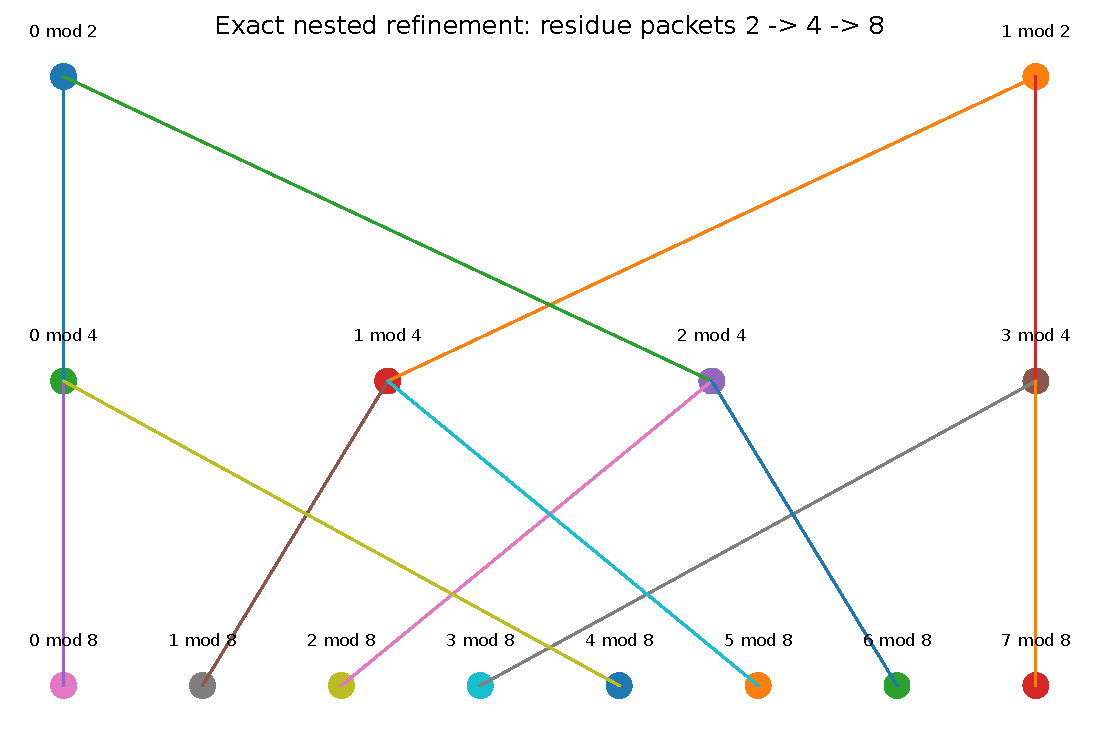
\includegraphics[width=0.94\textwidth]{01_nested_dyadic_refinement.pdf}
\caption{A nested residue hierarchy. Each residue modulo $2$ is the union of two residues modulo $4$, and each residue modulo $4$ is the union of two residues modulo $8$.}
\label{fig:refinement-tree}
\end{figure}
\subsection{Operator blocks across refinement}

For $T\in\End(X)$ and a packet system $\Pcal$, write
\[
T^{\Pcal}_{\beta\alpha}=P_\beta T P_\alpha.
\]

\begin{theorem}[Refinement of operator blocks]\label{thm:block_refinement}\label{thm:transfer-block-refinement}
Suppose that $\Qcal$ refines $\Pcal$ through $\rho$.  Then
\[
T^{\Pcal}_{ba}
=
\sum_{\substack{\rho(\beta)=b\\\rho(\alpha)=a}}
T^{\Qcal}_{\beta\alpha}.
\]
The matrix of $T$ in fine coordinates is related to the matrix in coarse coordinates by
\[
[T]_{\Pcal}
=
C_{\Pcal\leftarrow\Qcal}[T]_{\Qcal}J_{\Qcal\leftarrow\Pcal}.
\]
\end{theorem}

\begin{proof}
Expand the two coarse projectors into their children:
\[
P_bTP_a
=
\left(\sum_{\rho(\beta)=b}Q_\beta\right)
T
\left(\sum_{\rho(\alpha)=a}Q_\alpha\right).
\]
Distributing the finite sums gives the first identity.  For the coordinate identity, use
\[
[T]_{\Pcal}=\Acal_{\Pcal}T\Scal_{\Pcal}
\]
and insert
\[
I_X=\Scal_{\Qcal}\Acal_{\Qcal}.
\]
\end{proof}

\begin{corollary}[Support under refinement]\label{cor:block_support_refinement}
Under the hypotheses of \cref{thm:block_refinement}, a coarse block $T^{\Pcal}_{ba}$ is zero if and only if every fine descendant block
\[
T^{\Qcal}_{\beta\alpha}
\qquad
\bigl(\rho(\beta)=b,\ \rho(\alpha)=a\bigr)
\]
is zero.
\end{corollary}

\begin{proof}
If every fine block is zero, the coarse block is zero by \cref{thm:block_refinement}.  Conversely, suppose $P_bTP_a=0$.  Multiply on the left by $Q_\beta$ and on the right by $Q_\alpha$.  The child identities in \cref{thm:children_transitivity} give
\[
Q_\beta TQ_\alpha=0.
\]
\end{proof}

Thus refinement cannot hide an active transfer inside a zero coarse block.  It can only reveal where the active transfer sits among the descendants.

\begin{figure}[htbp]
\centering
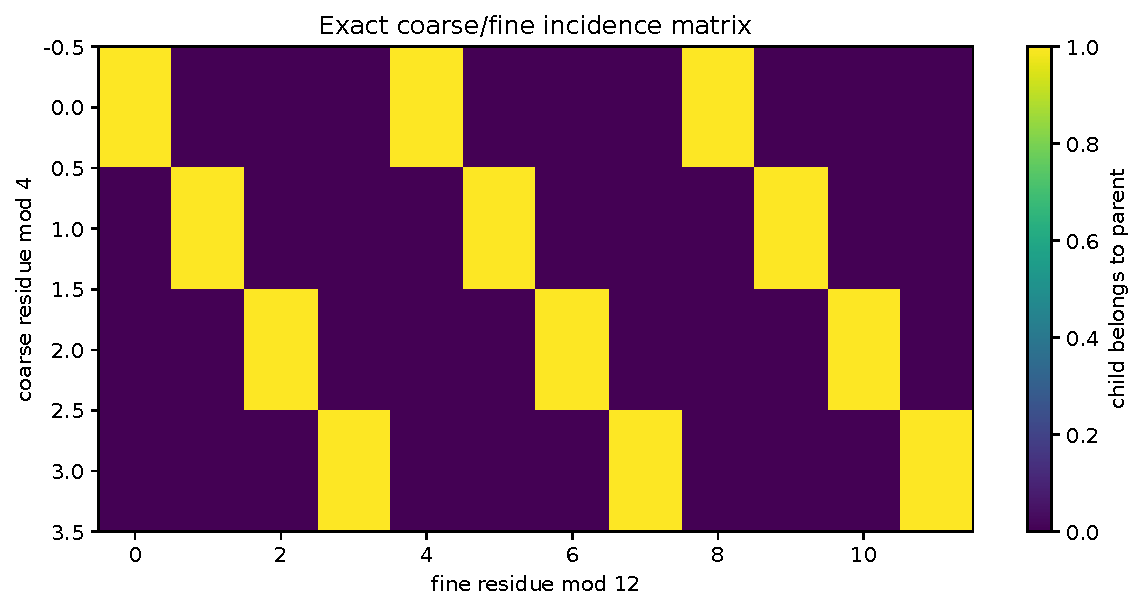
\includegraphics[width=0.92\textwidth]{03_refinement_incidence.pdf}
\caption{The incidence matrix $M_{r,s}=1$ when the fine residue $s$ belongs to the coarse residue $r$. Its rows implement exact fine-to-coarse packet aggregation.}
\label{fig:incidence}
\end{figure}
\subsection{Common refinements}

Two packet systems need not be comparable.  When their idempotents commute, their products give a common refinement.

\begin{theorem}[Common refinement of commuting packet systems]\label{thm:common_refinement}
Let $\Pcal=(P_\alpha)_{\alpha\in I}$ and $\Qcal=(Q_\beta)_{\beta\in J}$ be packet systems on $X$.  Assume
\[
P_\alpha Q_\beta=Q_\beta P_\alpha
\]
for all $\alpha$ and $\beta$.  Remove the zero operators from the family
\[
R_{\alpha\beta}=P_\alpha Q_\beta.
\]
The remaining operators form a packet system that refines both $\Pcal$ and $\Qcal$.  The same statement holds for any finite collection of pairwise commuting packet systems.
\end{theorem}

\begin{proof}
Commutativity gives
\[
R_{\alpha\beta}^2=P_\alpha^2Q_\beta^2=R_{\alpha\beta}.
\]
If $(\alpha,\beta)\ne(\alpha',\beta')$, then either $P_\alpha P_{\alpha'}=0$ or $Q_\beta Q_{\beta'}=0$, so the corresponding products annihilate one another.  Finally,
\[
\sum_{\alpha,\beta}R_{\alpha\beta}
=
\left(\sum_\alpha P_\alpha\right)
\left(\sum_\beta Q_\beta\right)
=I_X.
\]
For a fixed $\alpha$,
\[
P_\alpha
=P_\alpha\sum_\beta Q_\beta
=
\sum_\beta R_{\alpha\beta},
\]
and the same argument works for a fixed $\beta$.  Iteration proves the finite family statement.
\end{proof}

\begin{proposition}[Coarsest common refinement]\label{prop:coarsest_common_refinement}
Under the hypotheses of \cref{thm:common_refinement}, let $\Rcal$ be a packet system that refines both $\Pcal$ and $\Qcal$.  Then $\Rcal$ refines the nonzero product family $(P_\alpha Q_\beta)$.  Hence that product family is the coarsest packet system that refines both $\Pcal$ and $\Qcal$.
\end{proposition}

\begin{proof}
Let $R_\gamma$ be a packet in $\Rcal$.  Because $\Rcal$ refines $\Pcal$, there is a unique $\alpha$ with
\[
P_\alpha R_\gamma=R_\gamma.
\]
Likewise there is a unique $\beta$ with
\[
Q_\beta R_\gamma=R_\gamma.
\]
Therefore
\[
P_\alpha Q_\beta R_\gamma=R_\gamma.
\]
Every packet of $\Rcal$ lies in one product packet.  Summing the packets with the same pair of parents reconstructs that product packet.
\end{proof}

\begin{example}[A two level split]\label{ex:two_level_split}
Let
\[
X=X_{00}\oplus X_{01}\oplus X_{10}\oplus X_{11}.
\]
The four coordinate projections form a fine packet system.  The two sums
\[
P_0=Q_{00}+Q_{01},
\qquad
P_1=Q_{10}+Q_{11}
\]
form a coarse packet system.  If $x=(x_{00},x_{01},x_{10},x_{11})$, the coarse coordinates are
\[
(x_{00}+x_{01},x_{10}+x_{11})
\]
when the sums are interpreted inside the two coarse direct summands.  Fine analysis recovers the four entries exactly.  Nothing has been approximated.
\end{example}

\section{Residue coordinates and coprime factorization}\label{sec:residue}

Residue packets provide a model that works over every coefficient ring.  The character formula is a second description that needs stronger hypotheses.

\begin{definition}[Residue selector]\label{def:residue_selector}
Let $R$ be a commutative ring and let
\[
F(z)=\sum_{n\geq0}a_nz^n\in R[[z]].
\]
For $N\geq1$ and $0\leq j<N$, define
\[
(P_{N,j}F)(z)
=
\sum_{n\equiv j\pmod N}a_nz^n.
\]
\end{definition}

\begin{proposition}[Residue packet algebra]\label{prop:residue_algebra}\label{prop:residue-algebra}
For every commutative ring $R$, the operators $(P_{N,j})_{0\leq j<N}$ satisfy the identities below.  If $R$ is nonzero, they form a packet system on $R[[z]]$:
\[
P_{N,i}P_{N,j}=\delta_{ij}P_{N,j},
\qquad
\sum_{j=0}^{N-1}P_{N,j}=I.
\]
\end{proposition}

\begin{proof}
Every nonnegative integer belongs to one residue class modulo $N$.  A coefficient survives both $P_{N,i}$ and $P_{N,j}$ exactly when the two labels are equal to its residue.  Summing all selectors preserves every coefficient once.
\end{proof}

\subsection{Finite orthogonality certificates}

Let $U$ act on coefficient sequences by
\[
(UF)(z)=F(\omega z).
\]
If $\omega^N=1$, then $U^N=I$.

\begin{theorem}[Root-of-unity realization]\label{thm:root-of-unity}
Let $R$ be a commutative semiring, let $N>0$, and suppose
$\omega,\omega^\vee,\eta\in R$ satisfy $\omega^N=1$ and the finite
$N\times N$ Fourier orthogonality table
\[
\eta\sum_{k=0}^{N-1}(\omega^\vee)^{jk}\omega^{rk}
=
\begin{cases}
1,&r=j,\\
0,&r\ne j,
\end{cases}
\qquad 0\le j,r<N.
\]
Then
\[
\boxed{
P_{N,j}
=
\eta\sum_{k=0}^{N-1}(\omega^\vee)^{jk}U^k.
}
\]
In particular, if $R$ is a field, $N>0$, and $\omega$ is a primitive
$N$th root of unity, the certificate holds with
$\omega^\vee=\omega^{-1}$ and $\eta=N^{-1}$.
\end{theorem}

\begin{proof}
On the monomial $z^n$, the right-hand side acts by
\[
\eta\sum_{k=0}^{N-1}(\omega^\vee)^{jk}\omega^{nk}.
\]
The identity $\omega^N=1$ reduces this expression to the table entry indexed
by $r=n\bmod N$. The finite certificate therefore gives exactly the
coefficient mask defining $P_{N,j}$.
Over a field, the primitive-root geometric sum supplies the certificate.
\end{proof}

The field or orthogonality condition is essential. A primitive element of
order $N$ in a ring with zero divisors does not by itself force the off-diagonal
geometric sums to vanish. For example, in $\mathbb F_3\times\mathbb F_3$ the
element $(-1,1)$ has order two, but the second component of its nontrivial
character sum is nonzero. The division-free coefficient selector remains valid
without any Fourier certificate. This distinction becomes decisive at the
dyadic prime.


\subsection{The field specialization}
\begin{theorem}[Character realization]\label{thm:character_realization}
Let $\bbk$ be a field, assume that $N$ is nonzero in $\bbk$, and suppose that $\bbk$ contains a primitive $N$th root of unity $\omega$.  Define
\[
(UF)(z)=F(\omega z).
\]
Then
\[
P_{N,j}
=
\frac1N\sum_{k=0}^{N-1}\omega^{-jk}U^k.
\]
\end{theorem}

\begin{proof}
On $z^n$, the right side acts by the scalar
\[
\frac1N\sum_{k=0}^{N-1}\omega^{k(n-j)}.
\]
This is one when $n\equiv j\pmod N$ and zero otherwise by the geometric sum identity in the field $\bbk$.
\end{proof}

\begin{remark}[Two distinct constructions]\label{rem:selector_character}
The coefficient selector of \cref{def:residue_selector} uses no division.  The character formula in \cref{thm:character_realization} divides by $N$.  At a prime that divides $N$, the coefficient selector may remain integral even when the character average does not.
\end{remark}

\begin{theorem}[Nested residue refinement]\label{thm:residue_refinement}\label{thm:polyphase-refinement}
Let $N,M$ be positive integers with $N$ dividing $M$, and let $0\leq j<N$.  Then
\[
P_{N,j}
=
\sum_{\substack{0\leq s<M\\s\equiv j\pmod N}}P_{M,s}.
\]
When $R$ is nonzero, the packet system modulo $M$ refines the packet system modulo $N$.
\end{theorem}

\begin{proof}
An exponent $n$ satisfies $n\equiv j\pmod N$ exactly when its unique residue $s$ modulo $M$ satisfies $s\equiv j\pmod N$.
\end{proof}

\begin{example}[The shift graph of residue packets]\label{ex:residue_shift}
Multiplication by $z$ sends the residue packet $P_{N,j}R[[z]]$ into $P_{N,j+1}R[[z]]$, where the index is read modulo $N$.  Its packet graph is the directed cycle
\[
0\longrightarrow1\longrightarrow\cdots\longrightarrow N-1\longrightarrow0.
\]
Multiplication by a polynomial supported on a set of residues gives the corresponding finite set of phase shifts.  This is the simplest transfer graph behind a polyphase representation.
\end{example}

\begin{theorem}[Coprime factorization]\label{thm:crt_factorization}
Let $A$ and $B$ be coprime positive integers.  For each $j$ modulo $AB$, write
\[
j_A=j\pmod A,
\qquad
j_B=j\pmod B.
\]
Then
\[
P_{AB,j}=P_{A,j_A}P_{B,j_B}.
\]
Every pair $(j_A,j_B)$ occurs for one residue $j$ modulo $AB$.
\end{theorem}

\begin{proof}
A coefficient survives the product on the right exactly when its exponent satisfies both congruences.  The Chinese remainder theorem gives one residue class modulo $AB$ with those two coordinates.  The needed form of the theorem is standard and may be found in \cite{Lang2002}.
\end{proof}

\begin{corollary}[Dyadic and odd coordinates]\label{cor:dyadic_odd_coordinates}\label{thm:dyadic-odd}
Write $N=2^aM$ with $M$ odd.  Every residue packet modulo $N$ is the product of one packet modulo $2^a$ and one packet modulo $M$.
\end{corollary}

\begin{proof}
Apply \cref{thm:crt_factorization} to the coprime moduli $2^a$ and $M$.
\end{proof}

\begin{example}[Residues modulo twelve]\label{ex:mod_twelve}
The pair
\[
(j\pmod4,j\pmod3)=(3,1)
\]
corresponds to $j=7$ modulo $12$.  Hence
\[
P_{12,7}=P_{4,3}P_{3,1}.
\]
This factorization concerns addresses.  It does not say that the two factors have the same integral spectral behavior.
\end{example}

\begin{figure}[htbp]
\centering
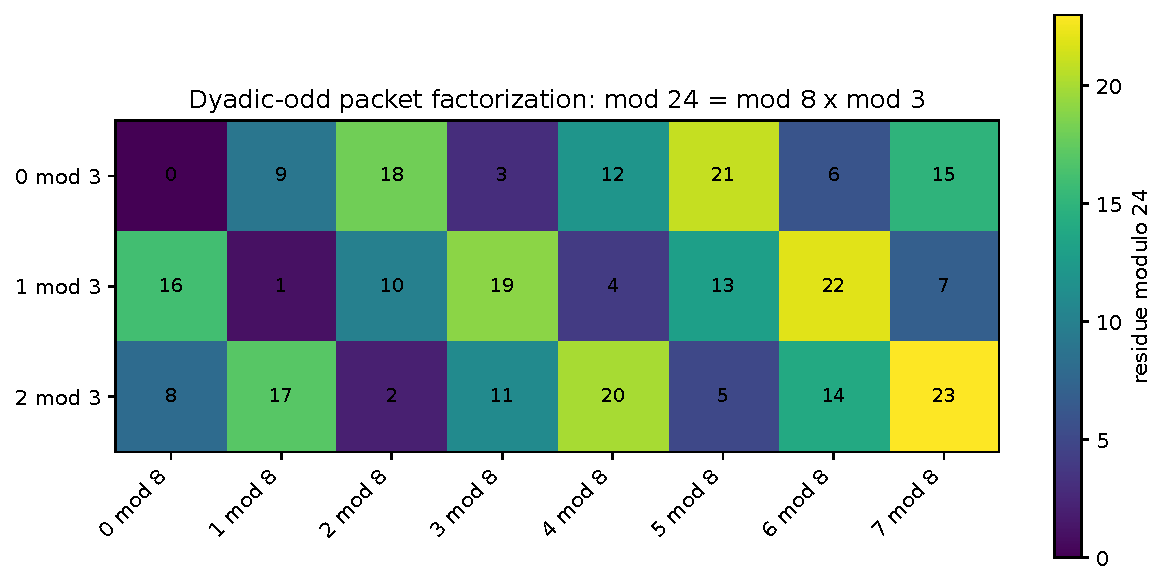
\includegraphics[width=0.95\textwidth]{02_crt_dyadic_odd_grid.pdf}
\caption{A composite residue packet is addressed by its dyadic and odd coordinates. The displayed mod-$24$ system is the product of mod $8$ and mod $3$.}
\label{fig:crt-grid}
\end{figure}
\section{Complete filtered transfer algebras}\label{sec:filtered}

Weighted inversion is most transparent in an abstract multiplicative filtration.  A discrete valuation ring is the main example.

\begin{definition}[Complete multiplicative filtration]\label{def:filtered_algebra}
A complete filtered algebra is a unital algebra $\Bcal$ with a decreasing sequence of two-sided ideals
\[
\Bcal=F^0\Bcal\supseteq F^1\Bcal\supseteq F^2\Bcal\supseteq\cdots
\]
such that
\[
F^r\Bcal\,F^s\Bcal\subseteq F^{r+s}\Bcal,
\qquad
\bigcap_{L\geq0}F^L\Bcal=0,
\]
and the natural map
\[
\Bcal\longrightarrow\varprojlim_L\Bcal/F^L\Bcal
\]
is an isomorphism.  A transfer term $N_e$ has declared weight $w(e)\geq1$ when
\[
N_e\in F^{w(e)}\Bcal.
\]
\end{definition}

If $\OO$ is a complete discrete valuation ring with uniformizer $\pi$, the filtration
\[
F^L\Bcal=\pi^L\Bcal
\]
is the standard example.  Basic facts about completeness in this setting are reviewed in \cite{Serre1979}.

\begin{theorem}[Weighted inverse]\label{thm:weighted_inverse}
Let $\Bcal$ be a complete filtered algebra.  Let $D\in\Bcal$ be invertible with
\[
D,D^{-1}\in F^0\Bcal.
\]
Let $E$ be a finite set and suppose
\[
T=D+\sum_{e\in E}N_e,
\qquad
N_e\in F^{w(e)}\Bcal,
\qquad
w(e)\geq1.
\]
Set
\[
A_e=D^{-1}N_e.
\]
For a word $\gamma=(e_1,\ldots,e_r)$, write
\[
A_\gamma=A_{e_r}\cdots A_{e_1},
\qquad
W(\gamma)=\sum_{j=1}^rw(e_j).
\]
The empty word has weight zero and contributes the identity.  Then $T$ is invertible and
\[
T^{-1}
=
\sum_\gamma(-1)^{|\gamma|}A_\gamma D^{-1}.
\]
The series converges in the filtration, and the term indexed by $\gamma$ belongs to $F^{W(\gamma)}\Bcal$.
\end{theorem}

\begin{proof}
Put
\[
A=\sum_{e\in E}A_e.
\]
Since left multiplication by $D^{-1}$ preserves the filtration, $A\in F^1\Bcal$.  Completeness gives the convergent Neumann series
\[
(I+A)^{-1}=\sum_{r\geq0}(-A)^r.
\]
Because $T=D(I+A)$,
\[
T^{-1}=(I+A)^{-1}D^{-1}.
\]
Expanding each power of $A$ gives the sum over words, with the rightmost edge acting first.  Multiplicativity of the filtration gives
\[
A_\gamma\in F^{W(\gamma)}\Bcal.
\]
For each $L$, only finitely many words have weight below $L$ because $E$ is finite and every edge has positive weight.  Thus the word expansion converges to the same inverse.
\end{proof}

The preceding formula does not yet use packet blocks.  When $D$ is packet diagonal and the terms $N_e$ are individual transfers, the words become directed paths.

\begin{theorem}[Block path formula]\label{thm:block_path_formula}
Let $\Pcal=(P_\alpha)_{\alpha\in I}$ be a finite packet system in a complete filtered algebra of operators.  Suppose
\[
D=\sum_\alpha P_\alpha D P_\alpha
\]
belongs to $\Bcal$ and is invertible on every packet.  Assume that the assembled inverse
\[
D^{-1}=\sum_\alpha D_\alpha^{-1}P_\alpha\in\Bcal=F^0\Bcal,
\qquad D_\alpha=P_\alpha DP_\alpha,
\]
where each packet inverse is extended by zero to the other packets.  Let the edge set be finite, assume $w(e)\geq1$ for every edge, and write
\[
N=\sum_{e:\alpha\to\beta}N_e,
\qquad
N_e=P_\beta N_eP_\alpha,
\qquad
N_e\in F^{w(e)}\Bcal.
\]
For an edge $e:\alpha\to\beta$, put
\[
A_e=(P_\beta DP_\beta)^{-1}N_e.
\]
Then the block from $P_\alpha X$ to $P_\beta X$ of $(D+N)^{-1}$ is
\[
P_\beta(D+N)^{-1}P_\alpha
=
\sum_{\gamma:\alpha\leadsto\beta}
(-1)^{|\gamma|}A_\gamma D_\alpha^{-1},
\]
where $D_\alpha=P_\alpha DP_\alpha$ and the sum runs over directed paths from $\alpha$ to $\beta$, including the empty path when $\alpha=\beta$.
\end{theorem}

\begin{proof}
The diagonal inverse is
\[
D^{-1}=\sum_\alpha D_\alpha^{-1}P_\alpha.
\]
The block $P_\beta D^{-1}NP_\alpha$ is nonzero only when there is a declared edge from $\alpha$ to $\beta$.  Repeated block multiplication shows that the $r$th power of $D^{-1}N$ is the sum over all directed paths of length $r$, with the operator factors ordered along the path.  Apply \cref{thm:weighted_inverse} and multiply on the right by the packet diagonal inverse.
\end{proof}

\begin{corollary}[Minimum path weight]\label{cor:minimum_path_weight}
For packets $\alpha$ and $\beta$, let $d(\alpha,\beta)$ be the least total weight of a directed path from $\alpha$ to $\beta$, with $d=\infty$ when no path exists.  Use the convention $F^\infty\Bcal=\bigcap_{L\geq0}F^L\Bcal=0$.  If $\alpha\ne\beta$, then
\[
P_\beta(D+N)^{-1}P_\alpha
\in
F^{d(\alpha,\beta)}\Bcal.
\]
If there is no path from $\alpha$ to $\beta$, the block is zero.
\end{corollary}

\begin{proof}
Every term in the block path formula is indexed by a path from $\alpha$ to $\beta$ and lies in the filtration level given by its total weight.  If no such path exists, the sum is empty.
\end{proof}

\begin{example}[A longer path that appears earlier]\label{ex:weighted_route}
Consider three packets $\alpha$, $\beta$, and $\gamma$.  Suppose there is a direct edge from $\alpha$ to $\gamma$ of weight three, together with edges
\[
\alpha\longrightarrow\beta,
\qquad
\beta\longrightarrow\gamma
\]
of weight one each.  The two edge route has total weight two, so it contributes to the inverse before the direct edge does.  This is why the truncation rule uses total weight rather than path length.  The lower bound in \cref{cor:minimum_path_weight} need not be an equality because several paths of the same weight may cancel.
\end{example}

\begin{corollary}[Acyclic transfer graph]\label{cor:acyclic_inverse}
If the packet transfer graph is acyclic, then $D^{-1}N$ is nilpotent.  The inverse in \cref{thm:block_path_formula} is a finite sum and does not require completeness of the filtration.
\end{corollary}

\begin{proof}
A finite acyclic directed graph has a bound on path length.  Every sufficiently long product of transfer blocks is therefore zero.  The Neumann series terminates.
\end{proof}

\begin{corollary}[Stability of inversion at finite precision]\label{cor:inverse_stability}
Let $T$ and $\widetilde T$ be invertible elements of $F^0\Bcal$.  If
\[
T-\widetilde T\in F^L\Bcal,
\]
then
\[
T^{-1}-\widetilde T^{-1}\in F^L\Bcal.
\]
\end{corollary}

\begin{proof}
Use the resolvent identity at zero in the form
\[
T^{-1}-\widetilde T^{-1}
=
T^{-1}(\widetilde T-T)\widetilde T^{-1}.
\]
Both inverse factors belong to $F^0\Bcal$, so the product lies in $F^L\Bcal$.
\end{proof}

\begin{corollary}[Exact finite precision truncation]\label{cor:finite_precision}
Under the hypotheses of \cref{thm:weighted_inverse}, define
\[
R_L
=
\sum_{W(\gamma)<L}(-1)^{|\gamma|}A_\gamma D^{-1}.
\]
Then
\[
T^{-1}-R_L\in F^L\Bcal,
\]
\[
TR_L-I\in F^L\Bcal,
\qquad
R_LT-I\in F^L\Bcal.
\]
Thus $R_L$ is the exact inverse in $\Bcal/F^L\Bcal$.
\end{corollary}

\begin{proof}
Every omitted word has weight at least $L$, so the difference from the full inverse lies in $F^L\Bcal$.  Multiplication by $T$ or by its inverse preserves membership in $F^L\Bcal$ under the stated filtration assumptions.  The two residual statements follow.
\end{proof}

\begin{example}[A triangular transfer]\label{ex:triangular_transfer}
Let $\OO$ be complete with uniformizer $\pi$, and consider
\[
T=
\begin{pmatrix}
1&\pi^a\\
0&1
\end{pmatrix}
\]
with $a\geq1$.  The only nontrivial transfer has weight $a$, and its square is zero.  Hence
\[
T^{-1}
=
\begin{pmatrix}
1&-\pi^a\\
0&1
\end{pmatrix}.
\]
At precision $L\leq a$, the transfer vanishes and the inverse is the identity modulo $\pi^L$.  At depth $a+1$, the off diagonal packet first becomes visible.
\end{example}

\paragraph{Two compatible word conventions.} The path expansion above labels a word in chronological order and writes its operator product in reverse order, so the first edge acts first.  The following finite-word contract uses written multiplication order.  Reversing all word labels identifies the sums over all words; individual path labels must retain their stated convention.  The two conventions do not change a weight or an inverse.

\subsection{Finite quotient and normed-ring realizations}

\subsubsection{Normalized edges and written-word convention}

Let $\OO$ be a complete discrete valuation ring with uniformizer $\pi$, fraction field $K$, and filtration
\[
F^m\cB=\pi^m\cB
\]
on an $\OO$-algebra $\cB$. Suppose
\[
T=D+H,
\]
where $D$ is invertible and the perturbation $H$ raises filtration. The symbol
$K$ is reserved for the fraction field.

A packet decomposition resolves $H=\sum_{e\in E}H_e$ and assigns a
certified filtration gain
\[
D^{-1}H_e\in F^{w(e)}\cB,
\qquad w(e)\in\Z_{>0}.
\]
Each $e$ is a directed transfer edge. For an ordered transfer word
\[
\gamma=(e_1,\ldots,e_r),
\]
define
\[
W(\gamma)=\sum_{j=1}^rw(e_j),
\qquad
A_\gamma=A_{e_1}\cdots A_{e_r},
\qquad A_e=D^{-1}H_e.
\]

\begin{figure}[htbp]
\centering
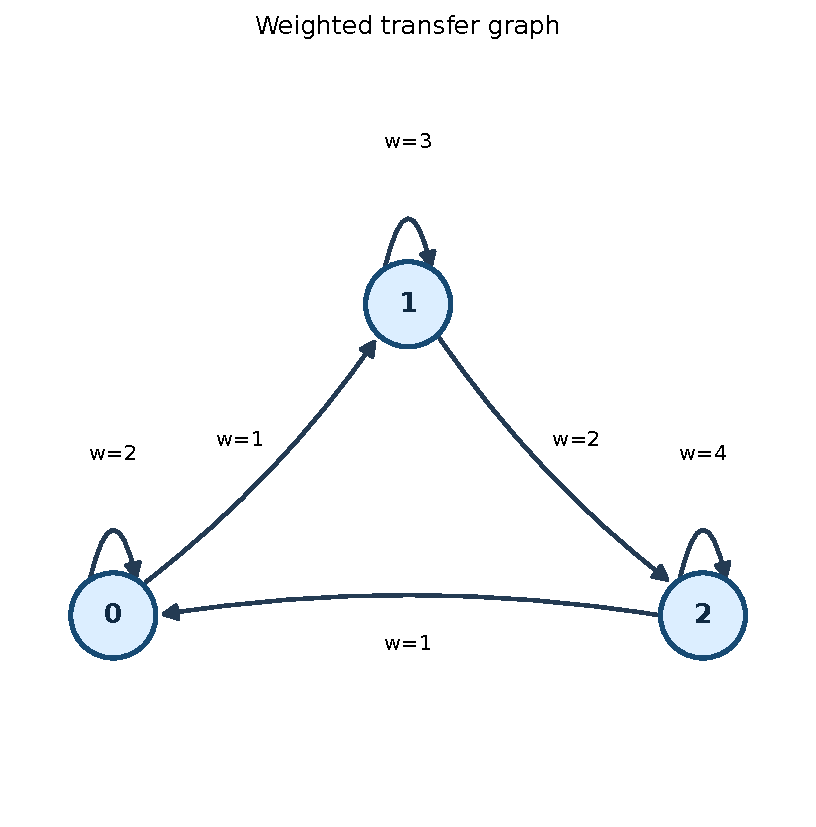
\includegraphics[width=0.87\textwidth]{04_weighted_transfer_graph.pdf}
\caption{A finite packet-transfer graph. Edge weights record filtration gain rather than merely the number of operator compositions.}
\label{fig:weighted-graph}
\end{figure}

\begin{theorem}[Certified weighted inverse]\label{thm:weighted-inverse}
Let $R$ be a possibly noncommutative ring, let $D^{-1}$ be a supplied
two-sided inverse of $D$, and put $A=D^{-1}H$.
\begin{enumerate}[label=(\alph*)]
\item If $A^r=0$, then $D+H$ has the two-sided inverse
\[
\boxed{(D+H)^{-1}=\left(\sum_{k=0}^{r-1}(-A)^k\right)D^{-1}.}
\]
\item If $R$ is a complete normed ring and $\lVert A\rVert<1$, then
$\sum_{k\ge0}(-A)^k$ converges and
\[
\boxed{(D+H)^{-1}=\left(\sum_{k\ge0}(-A)^k\right)D^{-1}.}
\]
\end{enumerate}
\end{theorem}

\begin{proof}
Factor
\[
T=D(I+A),
\qquad A=D^{-1}H.
\]
For a finite cutoff $r$, multiplication on either side gives the
noncommutative telescoping identity
\[
(I+A)\sum_{k=0}^{r-1}(-A)^k
=
\left(\sum_{k=0}^{r-1}(-A)^k\right)(I+A)
=1-(-A)^r.
\]
This proves (a). In (b), the strict norm bound makes the geometric series
summable. Continuity of multiplication passes the same identities to the
limit. Multiplication by $D^{-1}$ gives the displayed inverse in both orders.
\end{proof}

\begin{corollary}[Finite precision]\label{cor:finite-precision}
Let $F^\bullet R$ be a multiplicative decreasing filtration and let
$q_L:R\to R_L$ be a ring homomorphism that kills $F^L R$. Suppose
\[
H=\sum_{e\in E}H_e,
\qquad D^{-1}H_e\in F^{w(e)}R,
\qquad w(e)\ge1,
\]
with $E$ finite. Then $q_L(D^{-1}H)^L=0$, the finite sum in
\cref{thm:weighted-inverse}(a) is a two-sided inverse after applying $q_L$,
and its word expansion may discard every word of weight at least $L$.
More explicitly, for a length cutoff $N$, define
\[
S^{\mathrm{pr}}_{L,N}
=
\sum_{n=0}^{N-1}(-1)^n
\sum_{\substack{\gamma\in E^n\\W(\gamma)<L}}A_\gamma.
\]
Lean proves directly that $q_L(S^{\mathrm{pr}}_{L,N})$ equals the mapped
geometric inverse whenever $q_L(A^N)=0$, and hence is a two-sided inverse of
$q_L(I+A)$, where $A=\sum_eA_e=D^{-1}H$. With the supplied two-sided
inverse $D^{-1}$ of $D$, this gives the explicit two-sided inverse
\[
\boxed{q_L\!\left(S^{\mathrm{pr}}_{L,N}D^{-1}\right)}
\quad\text{of}\quad q_L(D+H).
\]
If every edge weight is at least $m$ and $L\le mN$, then the nilpotence
condition follows from the filtration data because
$m|\gamma|\le W(\gamma)$. For $m>0$, the executable choice
$N=\lceil L/m\rceil$ satisfies $L\le mN$; this elementary ceiling inequality
is also proved in Lean. The choice $m=1,N=L$ gives the standard cutoff.
In the DVR example $q_L:R\to R/\pi^L R$, this reads
\[
q_L(T)^{-1}
=
q_L\!\left(\sum_{W(\gamma)<L}
(-1)^{|\gamma|}A_\gamma D^{-1}\right).
\]
\end{corollary}

Here $A_\gamma=(D^{-1}H_{e_1})\cdots(D^{-1}H_{e_r})$ in the written
order. Multiplicativity places it in $F^{W(\gamma)}R$, so the quotient kills
it when $W(\gamma)\ge L$. Positive weights also imply
$|\gamma|\le W(\gamma)$, making the retained search finite.

No unrestricted convergence assertion for every complete filtered algebra is
used in the formal contract. Such an assertion needs a separately specified
topology and completeness theorem. The release proves the finite-quotient
result above and the complete-normed contraction specialization.

\begin{figure}[htbp]
\centering
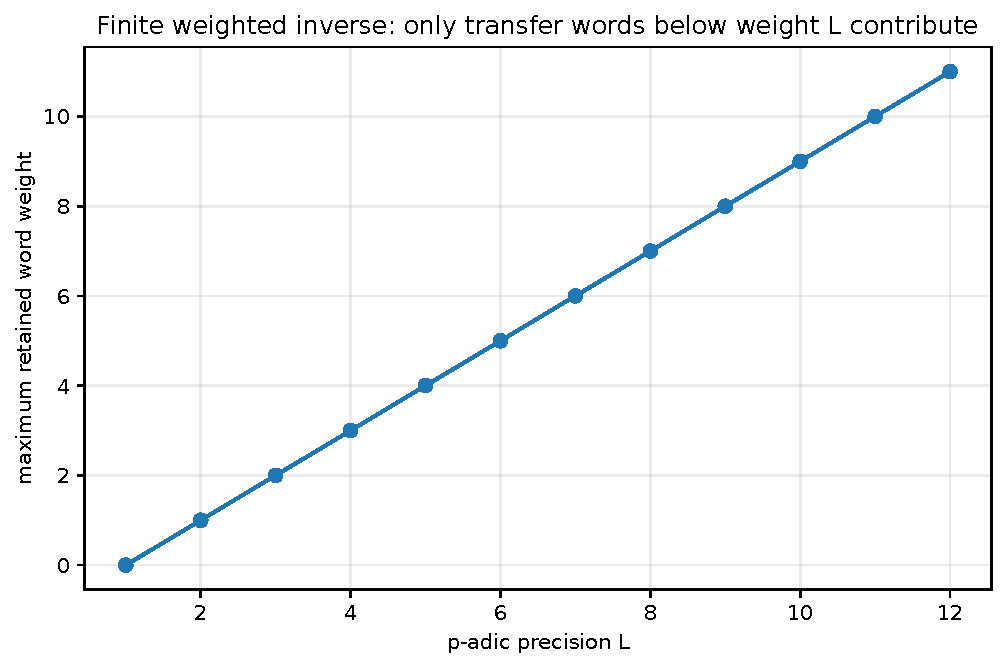
\includegraphics[width=0.84\textwidth]{06_filtered_inverse_depth.pdf}
\caption{At precision $L$, weighted inversion requires only transfer words whose cumulative weight is below $L$.}
\label{fig:inverse-depth}
\end{figure}


\section{Rational weighted transfer series}\label{sec:path_series}

A finite weighted graph records which path terms can occur in the inverse.  Its path counts have a rational generating function.

\begin{definition}[Weighted transfer series]\label{def:transfer_series}
Let $G$ be a finite directed multigraph.  Give every edge $e$ a positive integer weight $w(e)$ and a scalar multiplicity $m(e)$ in a field $\bbk$.  Define the polynomial adjacency matrix
\[
A(t)_{ij}
=
\sum_{e:i\to j}m(e)t^{w(e)}.
\]
For column vectors $u$ and $v$, define
\[
Z_{u,v}(t)
=
\sum_{n\geq0}a_nt^n,
\]
where $a_n$ is the total multiplicity of paths from the vertices selected by $u$ to the vertices selected by $v$ with total weight $n$.
\end{definition}

\begin{theorem}[Rationality of the transfer series]\label{thm:transfer_rationality}
The weighted transfer series satisfies
\[
Z_{u,v}(t)
=
u^{\mathsf T}(I-A(t))^{-1}v.
\]
It is a rational function whose denominator divides
\[
\det(I-A(t)).
\]
\end{theorem}

\begin{proof}
Since every entry of $A(t)$ has zero constant term, the inverse exists in the formal power series ring and
\[
(I-A(t))^{-1}=\sum_{r\geq0}A(t)^r.
\]
The $(i,j)$ entry of $A(t)^r$ is the sum of the monomials attached to all paths of length $r$ from $i$ to $j$.  Summing over $r$ records paths of every length.  Multiplication by the endpoint vectors gives the stated series.  The adjugate formula gives
\[
(I-A(t))^{-1}
=
\frac{\operatorname{adj}(I-A(t))}{\det(I-A(t))},
\]
so every entry is rational.
\end{proof}

\begin{corollary}[Recurrence for path counts]\label{cor:path_recurrence}
Write
\[
Z_{u,v}(t)=\frac{P(t)}{Q(t)},
\qquad
Q(t)=1+q_1t+\cdots+q_dt^d.
\]
Then, for every $n>\deg P$,
\[
a_n+q_1a_{n-1}+\cdots+q_da_{n-d}=0.
\]
\end{corollary}

\begin{proof}
Compare coefficients in the identity
\[
Q(t)Z_{u,v}(t)=P(t).
\]
Beyond the degree of $P$, the coefficient on the right is zero.
\end{proof}

\begin{corollary}[Several independent weights]\label{cor:multigraded_series}
Suppose every edge has a weight vector
\[
w(e)=(w_1(e),\ldots,w_r(e))\in\mathbb N^r\setminus\{0\}.
\]
Replace $t^{w(e)}$ by
\[
t_1^{w_1(e)}\cdots t_r^{w_r(e)}.
\]
The resulting multigraded transfer series is rational in $t_1,\ldots,t_r$.
\end{corollary}

\begin{proof}
The same matrix inverse proof works over the formal power series ring in several variables.  The adjugate formula gives rationality.
\end{proof}

The multigraded form is useful when dyadic depth, odd depth, and another filtration are tracked separately rather than collapsed into one number.

\begin{example}[A transfer series with one loop]\label{ex:simple_transfer_series}
Take vertices $0$, $1$, and $2$.  Give the edge $0\to1$ weight one, the loop $1\to1$ weight two, and the edge $1\to2$ weight one.  Every path from $0$ to $2$ uses the first and last edges and may traverse the loop any number of times.  Hence
\[
Z_{0,2}(t)
=
t^2(1+t^2+t^4+\cdots)
=
\frac{t^2}{1-t^2}.
\]
There is one path at every positive even weight and no path at an odd weight.  The denominator records the increase of two units produced by the loop.
\end{example}

\subsection{Automatic finite-graph construction}

Let $G$ be a finite directed graph with positive integer edge weights. Define the polynomial adjacency matrix
\[
A(t)_{ij}
=
\sum_{e:i\to j}t^{w(e)},
\]
where parallel edges are distinct elements of the finite edge type and are
therefore counted with their full multiplicity.

For fixed start and target vertices $s,t$, define
\[
Z_{s,t}(t)
=
\sum_{n\ge0}a_n(s,t)t^n,
\]
where $a_n(s,t)$ counts directed walks from $s$ to $t$ with total weight $n$.
Vertices and edges may repeat. Thus ``path zeta'' is retained as the name of
the series and Lean API, but no simple-path restriction is intended.

\begin{theorem}[Automatic finite-graph transfer-zeta rationality]\label{thm:transfer-zeta}
Assume the vertex and edge sets are finite and every edge has positive integer
weight. For every $n$, exact enumeration of edge tuples of lengths at most
$n$, followed by endpoint and total-weight filtering, returns $a_n(s,t)$.
These coefficients obey the first-edge recurrence
\[
a_n(s,t)
=
\mathbf 1_{s=t,\,n=0}
+\sum_{\substack{e:\,\operatorname{source}(e)=s\\w(e)\le n}}
a_{n-w(e)}(\operatorname{target}(e),t).
\]
Let
\[
T(t)=I-A(t),\qquad
Q(t)=\det T(t),\qquad
P_{s,t}(t)=\operatorname{adj}(T(t))_{s,t}.
\]
Then $Q(0)=1$, hence $Q\ne0$ and $Q$ is a unit in $\Z[[t]]$, and the
independently enumerated walk series satisfies
\[
\boxed{
Z_{s,t}(t)=Q(t)^{-1}P_{s,t}(t),
\qquad
Q(t)Z_{s,t}(t)=P_{s,t}(t)
}
\quad\text{in }\Z[[t]].
\]
\end{theorem}

\begin{proof}
Every edge has weight at least one, so a word of weight $n$ has length at
most $n$. The enumerator therefore searches a finite set containing every
contributing walk, and its filters are exactly the defining predicates for
$a_n$. Removing the first edge gives the displayed disjoint decomposition
into the empty diagonal walk and the first-edge tails. In matrix form this is
\[
Z=I+AZ,
\qquad (I-A)Z=I.
\]
Positive weights give $A(0)=0$, so $T(0)=I$ and
$Q(0)=\det(I)=1$. The two adjugate identities
\[
T\operatorname{adj}(T)=Q I,
\qquad
\operatorname{adj}(T)T=Q I
\]
remain valid after inclusion into $\Z[[t]]$. Multiplying the adjugate by the
formal-series inverse of $Q$ constructs a two-sided inverse of $T$.
Uniqueness of the inverse identifies that construction with the independently
enumerated matrix $Z$, yielding the entrywise formulas.
\end{proof}

This is the finite transfer-matrix method of \cite{Stanley2012}, but here its
determinant, adjugate, normalization, first-edge recurrence, and identification
with the enumerated series are all formalized. The older API accepting an
independently supplied normalized coefficient identity $QZ=P$ is retained for
external certificates; it is no longer needed to obtain rationality for the
finite graph defined above. The Python companion performs an exact symbolic
construction as an independent executable cross-check.

\begin{corollary}[Linear recurrence]\label{cor:zeta-recurrence}
With the canonical polynomials from \cref{thm:transfer-zeta}, write
\[
Q(t)=\sum_kq_kt^k,
\qquad
Z_{s,t}(t)=\sum_{n\ge0}a_n(s,t)t^n.
\]
Then the walk counts satisfy the constant-coefficient recurrence determined by
$Q$ after the finite initial range contributed by $P_{s,t}$:
\[
\boxed{
\sum_{k=0}^{n}q_k a_{n-k}(s,t)=0
\qquad\bigl(n>\deg P_{s,t}\bigr).
}
\]
\end{corollary}

\begin{figure}[htbp]
\centering
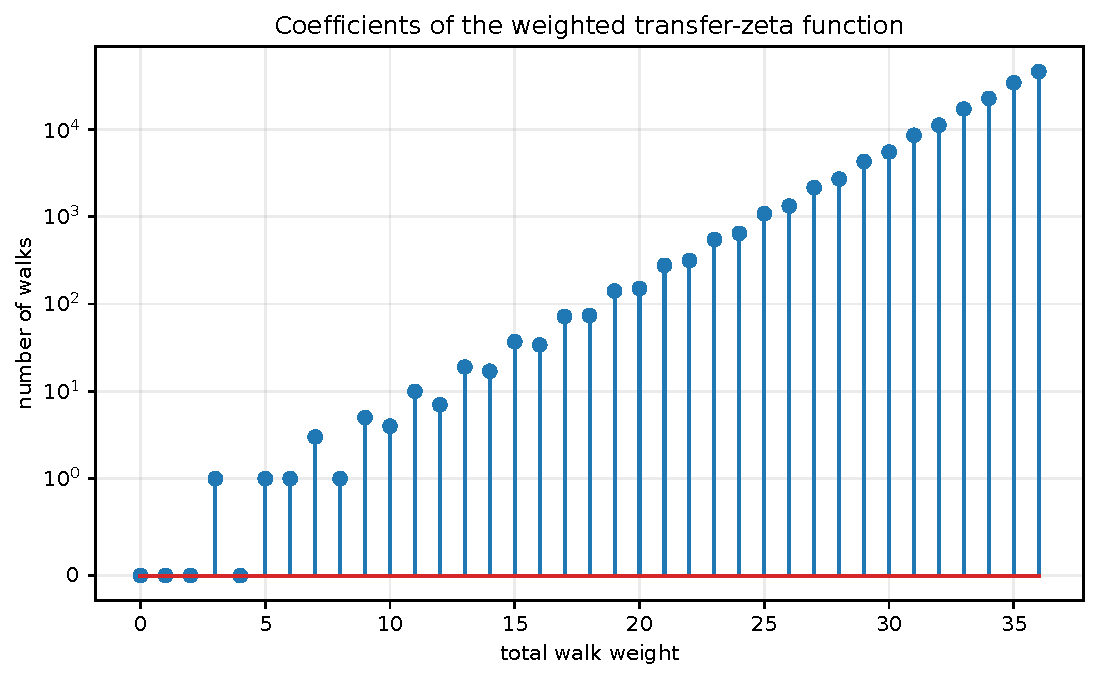
\includegraphics[width=0.88\textwidth]{05_path_zeta_coefficients.pdf}
\caption{The walk counts for one weighted graph. The exact generating function is rational, so these counts satisfy a finite linear recurrence.}
\label{fig:zeta-counts}
\end{figure}

\begin{example}[A computed transfer zeta]
For the graph used in the numerical companion, the walk series from packet $0$ to packet $2$ is
\[
Z_{0,2}(t)
=
\frac{t^3}{1-t^2-t^3-2t^4+t^5+t^6+t^7-t^9}.
\]
The first nonzero coefficients are
\[
1,1,1,3,1,5,4,10,7,19,17,37,\ldots
\]
at their corresponding weights. Direct enumeration through weight $30$ agrees coefficient by coefficient with the rational expansion.
\end{example}


\section{Rational spectral projectors and resultant bounds}\label{sec:resultant}

Let $\OO$ be a discrete valuation ring with fraction field $K$ and uniformizer $\pi$.  Let $\Lambda$ be a finite free $\OO$ module and put
\[
V=K\otimes_{\OO}\Lambda.
\]
Suppose $A\in\End_{\OO}(\Lambda)$.

\begin{theorem}[Bézout spectral projector]\label{thm:bezout_projector}
Assume that
\[
\chi_A(x)=f(x)g(x)
\]
with monic polynomials $f,g\in\OO[x]$ that are coprime in $K[x]$.  Choose $u,v\in\OO[x]$ and a nonzero $r\in\OO$ such that
\[
u(x)f(x)+v(x)g(x)=r.
\]
Then
\[
E_f=r^{-1}v(A)g(A)
\]
is the projector of $V$ onto $\Ker f(A)$ along $\Ker g(A)$.  In particular,
\[
E_f^2=E_f,
\qquad
rE_f\in\End_{\OO}(\Lambda).
\]
\end{theorem}

\begin{proof}
Cayley Hamilton gives
\[
f(A)g(A)=0.
\]
If $x\in\Ker f(A)$, then the Bézout identity gives
\[
v(A)g(A)x=rx,
\]
so $E_fx=x$.  If $x\in\Ker g(A)$, then $E_fx=0$.  The same identity gives the direct sum decomposition
\[
V=\Ker f(A)\oplus\Ker g(A).
\]
Indeed, every $x\in V$ is the sum of
\[
r^{-1}v(A)g(A)x\in\Ker f(A)
\]
and
\[
r^{-1}u(A)f(A)x\in\Ker g(A).
\]
Thus $E_f$ is the stated projector and is idempotent.  The formula for $rE_f$ has coefficients in $\OO$, so it preserves $\Lambda$.
\end{proof}

\begin{theorem}[Several coprime spectral packets]\label{thm:several_projectors}
Assume
\[
\chi_A(x)=\prod_{i=1}^rf_i(x),
\]
where the monic factors $f_i\in\OO[x]$ are pairwise coprime in $K[x]$.  Put
\[
g_i=\prod_{j\ne i}f_j.
\]
There are complementary projectors $E_i$ with
\[
\im E_i=\Ker f_i(A),
\qquad
\sum_iE_i=I,
\qquad
E_iE_j=0
\quad(i\ne j).
\]
One may choose $E_i$ so that
\[
\Res(f_i,g_i)E_i\in\End_{\OO}(\Lambda)
\]
up to multiplication of the resultant by a unit.
\end{theorem}

\begin{proof}
Apply \cref{thm:bezout_projector} to the factorization $\chi_A=f_ig_i$.  The resulting projector is one on $\Ker f_i(A)$ and zero on every $\Ker f_j(A)$ with $j\ne i$.  The direct sum decomposition follows from the polynomial Chinese remainder theorem.  The orthogonality and sum identities follow by evaluating the corresponding idempotents in $K[x]/(\chi_A)$.  The Sylvester Bézout relation for $(f_i,g_i)$ gives the stated denominator bound.
\end{proof}

\begin{corollary}[Resultant denominator bound]\label{cor:resultant_bound}
Under the hypotheses of \cref{thm:bezout_projector}, one may take
\[
r=\Res(f,g)
\]
up to multiplication by a unit.  Therefore
\[
\pi^{\val_\pi(\Res(f,g))}E_f\Lambda\subseteq\Lambda.
\]
\end{corollary}

\begin{proof}
The Sylvester matrix construction gives a Bézout relation with right side equal to the resultant.  Apply \cref{thm:bezout_projector}.  Standard facts about resultants may be found in \cite{Lang2002,GohbergLancasterRodman2009}.
\end{proof}

\begin{example}[A resultant bound that is not exact]\label{ex:loose_resultant}
Let
\[
A=\diag(0,\pi^s)
\]
on the standard lattice $\Lambda=\OO^2$.  The factors $x$ and $x-\pi^s$ have resultant $-\pi^s$, up to the harmless choice of resultant order, but the two spectral projectors are the integral coordinate projectors.  Their exact separation weight is zero.  The resultant sees the closeness of the two eigenvalues.  It does not see that the chosen lattice already splits along their eigenspaces.
\end{example}

\subsection{Evaluated certificates and explicit lattice action}

\subsubsection{Minimal evaluated B\'ezout identities}

Let $\OO$ be a DVR, $K=\Frac(\OO)$, and $A\in\End_\OO(\Lambda)$ for a finite free lattice $\Lambda$. Suppose the characteristic polynomial factors over $\OO$ as
\[
\chi_A(x)=f(x)g(x),
\]
where $f$ and $g$ are coprime over $K[x]$.

\begin{theorem}[Evaluated B\'ezout spectral projector]\label{thm:bezout-projector}
Let $F,G,U,V\in\End_K(\Lambda\otimes_\OO K)$ and let $r\in K^\times$.
Suppose
\[
UF+VG=rI,
\qquad FG=0,
\qquad FG=GF,
\qquad GU=UG.
\]
Put $N=VG$. Then
\[
\boxed{N^2=rN.}
\]
Consequently the operator
\[
\boxed{
E=r^{-1}VG
}
\]
is idempotent, acts as the identity on $\ker F$, and acts as zero on
$\ker G$. If $V$ and $G$ preserve $\Lambda$, then
\[
rE=VG\in\End_\OO(\Lambda).
\]
\end{theorem}

\begin{proof}
The B\'ezout identity gives $N=rI-UF$. The two stated commutation relations
and $FG=0$ give
\[
N(UF)=VGUF=VUGF=VUFG=0.
\]
Therefore
\[
N^2=N(rI-UF)=rN.
\]
Since $r\ne0$, $E^2=r^{-2}N^2=E$. If $Fx=0$, the evaluated B\'ezout
identity gives $VGx=rx$, hence $Ex=x$. If $Gx=0$, then $Ex=0$.
The lattice assertion follows directly from $rE=VG$.
\end{proof}

The denominator-free equality $N^2=rN$ uses neither $r\ne0$ nor the other
pairwise commutation relations that hold in the polynomial application. The
normalization to $E$ uses $r\ne0$; action on $\ker F$ uses only the B\'ezout
identity and $r\ne0$, while vanishing on $\ker G$ is immediate from $N=VG$.
The bundled Lean certificate records all pairwise commutations as convenient
evaluated polynomial data, but the minimal theorems expose only the hypotheses
they consume.

For the polynomial application, one supplies $F=f(A)$, $G=g(A)$,
$U=u(A)$, and $V=v(A)$. A B\'ezout or resultant identity
$uf+vg=r$ evaluates to the first certificate, while
$(fg)(A)=0$ supplies the second; when $fg=\chi_A$, this last equality is
Cayley--Hamilton. Standard B\'ezout, resultant, and DVR facts are recalled
from \cite{Lang2002,Serre1979}. The formal theorem begins with the evaluated
certificate. It does not infer exact action merely from nilpotence of
$f(A)$ or $g(A)$, which would be insufficient.

\begin{definition}[Separation weight]\label{def:separation-weight}
For a rational projector $E$ and a specified $\OO$-lattice $\Lambda$, provided
at least one clearing exponent exists, define
\[
s_{\pi,\Lambda}(E)
=
\min\{s\ge0:\pi^sE(\Lambda)\subseteq\Lambda\}.
\]
If the evaluated certificate arises from integral $v,g$ and
$r=u\pi^s$ with $u^{-1}$ preserving the lattice, then
\cref{thm:bezout-projector} gives the upper bound
\[
s_{\pi,\Lambda}(E)\le s=\val_\pi(r).
\]
Indeed,
\[
\boxed{\pi^sE=u^{-1}VG}
\]
preserves $\Lambda$. The minimal Lean theorem needs only the lattice action of
$u^{-1}$; its bundled lattice-unit wrapper records both $u$ and $u^{-1}$,
rather than treating every nonzero fraction-field scalar as an integral unit.
Existence of a clearing exponent is an explicit hypothesis, not a consequence
of the notation. Once one exists, the least one is obtained by well-ordering.
Clearing exponents are upward closed provided multiplication by $\pi$
preserves the lattice.
\end{definition}

\subsubsection{Certificate-level precision delay}

\begin{theorem}[Projector precision delay]\label{thm:precision-delay}
Let $E$ be a rational projector with $\pi^sE(\Lambda)\subseteq\Lambda$. If
\[
x\equiv y\pmod{\pi^{m+s}\Lambda},
\]
then
\[
Ex\equiv Ey\pmod{\pi^m\Lambda}.
\]
Thus $m+s$ input digits suffice to determine $m$ output digits of the projected packet.
\end{theorem}

\begin{proof}
Write $x-y=\pi^{m+s}z$. Since $\pi^sE(z)\in\Lambda$,
\[
E(x-y)=\pi^m\bigl(\pi^sE(z)\bigr)\in\pi^m\Lambda.
\]
\end{proof}

The theorem makes delayed separation quantitative. A packet with weight $s$ is not absent; it requires $s$ additional digits before it can be reconstructed to the same output precision.


\section{Exact lattice separation}\label{sec:lattice}

The exact denominator belongs to the pair consisting of the rational packet decomposition and the integral lattice.

\begin{definition}[Lattice packet data]\label{def:lattice_packet}
Let
\[
V=\bigoplus_{\alpha\in I}V_\alpha
\]
be a finite direct sum over $K$, with packet projectors $E_\alpha$.  Let $\Lambda\subseteq V$ be an $\OO$ lattice.  Put
\[
\Lambda_\alpha=\Lambda\cap V_\alpha,
\qquad
\Lambda_{\mathrm{split}}=\bigoplus_\alpha\Lambda_\alpha,
\]
and define the gluing module
\[
G_{\Lambda,\Pcal}
=
\Lambda/\Lambda_{\mathrm{split}}.
\]
The separation weight of $E_\alpha$ is
\[
s_\Lambda(E_\alpha)
=
\min\{s\geq0:\pi^sE_\alpha\Lambda\subseteq\Lambda\}.
\]
The global separation weight is
\[
s_\Lambda(\Pcal)=\max\bigl(\{0\}\cup\{s_\Lambda(E_\alpha):\alpha\in I\}\bigr).
\]
For a finite torsion $\OO$ module $G$, write $\expn_\pi(G)$ for the least $s$ such that $\pi^sG=0$.
\end{definition}

The module $G_{\Lambda,\Pcal}$ is finite because $\Lambda_{\mathrm{split}}$ and $\Lambda$ are full lattices in the same vector space.

\begin{theorem}[Gluing module and exact separation weight]\label{thm:gluing_weight}
With the notation of \cref{def:lattice_packet}, the map
\[
\Phi:G_{\Lambda,\Pcal}
\longrightarrow
\bigoplus_{\alpha\in I}E_\alpha\Lambda/\Lambda_\alpha,
\qquad
[x]\longmapsto(E_\alpha x+\Lambda_\alpha)_\alpha
\]
is injective, and every coordinate projection of its image is surjective.  We also have
\[
\boxed{
\expn_\pi(G_{\Lambda,\Pcal})
=
s_\Lambda(\Pcal).
}
\]
If
\[
G_{\Lambda,\Pcal}
\cong
\bigoplus_{j=1}^r\OO/\pi^{a_j}\OO
\]
with $a_1\leq\cdots\leq a_r$, then
\[
s_\Lambda(\Pcal)=\max\bigl(\{0\}\cup\{a_j:1\leq j\leq r\}\bigr).
\]
\end{theorem}

\begin{proof}
If $x\in\Lambda$ maps to zero, then $E_\alpha x\in\Lambda_\alpha$ for every $\alpha$.  Since
\[
x=\sum_\alpha E_\alpha x,
\]
we have $x\in\Lambda_{\mathrm{split}}$.  Thus $\Phi$ is injective.  The coordinate map onto $E_\alpha\Lambda/\Lambda_\alpha$ is surjective by the definition of $E_\alpha\Lambda$.

Let $s=s_\Lambda(\Pcal)$.  For every $x\in\Lambda$ and every $\alpha$,
\[
\pi^sE_\alpha x\in\Lambda_\alpha.
\]
Hence
\[
\pi^sx=\sum_\alpha\pi^sE_\alpha x\in\Lambda_{\mathrm{split}},
\]
so $\pi^sG_{\Lambda,\Pcal}=0$.  This proves
\[
\expn_\pi(G_{\Lambda,\Pcal})\leq s.
\]
If $d<s$, then for some $\alpha$ there is an $x\in\Lambda$ with
\[
\pi^dE_\alpha x\notin\Lambda_\alpha.
\]
The class $\pi^d[x]$ is therefore nonzero in the gluing module.  Thus $\pi^d$ does not annihilate the gluing module, and equality follows.  The final formula is the usual description of the exponent through Smith normal form.
\end{proof}

\begin{corollary}[Total gluing and worst precision]\label{cor:length_and_weight}
If
\[
G_{\Lambda,\Pcal}
\cong
\bigoplus_{j=1}^r\OO/\pi^{a_j}\OO,
\]
then
\[
\length_{\OO}(G_{\Lambda,\Pcal})
=
\sum_{j=1}^ra_j,
\qquad
s_\Lambda(\Pcal)=\max\bigl(\{0\}\cup\{a_j:1\leq j\leq r\}\bigr).
\]
Thus the lattice index measures the total amount of gluing, while the separation weight measures the worst precision loss in one direction.
\end{corollary}

\begin{proof}
The length and exponent of a finite module are read directly from its Smith decomposition.  Apply \cref{thm:gluing_weight}.
\end{proof}

\begin{corollary}[Two complementary packets]\label{cor:binary_gluing}
Suppose
\[
V=V_1\oplus V_2
\]
with projector $E$ onto $V_1$ and complementary projector $I-E$.  Then
\[
\Lambda/(\Lambda_1\oplus\Lambda_2)
\cong
E\Lambda/\Lambda_1
\cong
(I-E)\Lambda/\Lambda_2.
\]
Consequently
\[
s_\Lambda(E)=s_\Lambda(I-E)
=
\expn_\pi\bigl(\Lambda/(\Lambda_1\oplus\Lambda_2)\bigr).
\]
\end{corollary}

\begin{proof}
Map $x\in\Lambda$ to $Ex+\Lambda_1$.  Its kernel consists of the $x$ for which $Ex\in\Lambda_1$.  In that case
\[
(I-E)x=x-Ex\in\Lambda\cap V_2=\Lambda_2,
\]
so the kernel is $\Lambda_1\oplus\Lambda_2$.  The map is surjective by definition.  The complementary map is handled in the same way.  The equality of weights follows from \cref{thm:gluing_weight}.
\end{proof}

\begin{corollary}[Integral splitting criterion]\label{cor:integral_split}
Every packet projector preserves $\Lambda$ if and only if
\[
\Lambda=\bigoplus_\alpha(\Lambda\cap V_\alpha).
\]
Equivalently,
\[
s_\Lambda(\Pcal)=0
\quad\Longleftrightarrow\quad
G_{\Lambda,\Pcal}=0.
\]
\end{corollary}

\begin{proof}
If every projector preserves $\Lambda$, then
\[
x=\sum_\alpha E_\alpha x
\]
expresses every $x\in\Lambda$ as a sum of vectors in $\Lambda_\alpha$.  The converse is immediate because each projector is the identity on one direct summand and zero on the others.  The final equivalence follows from \cref{thm:gluing_weight}.
\end{proof}

\subsection{Refinement and separation weight}

A finer rational packet system imposes more integral splitting conditions.

\begin{theorem}[Gluing exact sequence under refinement]\label{thm:gluing_refinement}
Let $\Qcal=(Q_\beta)$ refine $\Pcal=(P_\alpha)$ on $V$, and let $\Lambda$ be a lattice.  Define
\[
\Lambda_{\Pcal}
=
\bigoplus_\alpha(\Lambda\cap P_\alpha V),
\qquad
\Lambda_{\Qcal}
=
\bigoplus_\beta(\Lambda\cap Q_\beta V).
\]
Then
\[
\Lambda_{\Qcal}\subseteq\Lambda_{\Pcal}\subseteq\Lambda
\]
and there is a short exact sequence
\[
0
\longrightarrow
\Lambda_{\Pcal}/\Lambda_{\Qcal}
\longrightarrow
\Lambda/\Lambda_{\Qcal}
\longrightarrow
\Lambda/\Lambda_{\Pcal}
\longrightarrow0.
\]
In particular,
\[
\boxed{
s_\Lambda(\Pcal)\leq s_\Lambda(\Qcal).
}
\]
\end{theorem}

\begin{proof}
Every fine packet space lies in its parent packet space, so every element of $\Lambda_{\Qcal}$ belongs to $\Lambda_{\Pcal}$.  The displayed exact sequence is the standard quotient sequence for nested submodules.  The exponent of a quotient cannot exceed the exponent of the module from which it is obtained.  Apply \cref{thm:gluing_weight} to the two gluing modules.
\end{proof}

\begin{example}[Strict growth under refinement]\label{ex:strict_weight_growth}
Take the standard lattice $\mathbb Z_2^2$ and the involution from \cref{prop:sign_projectors}.  The one packet system $(I)$ has weight zero.  Refining it into the two rational sign packets produces weight one.  The coarse lattice is already split because there is only one summand.  The fine eigenspaces are glued together by one dyadic digit.
\end{example}

\begin{remark}[Strict growth can occur]\label{rem:strict_growth}
A coarse packet family may preserve the lattice even though a fine spectral split does not.  Refinement can reveal rational directions that are glued together integrally.  The weight records the extra depth needed to separate them.
\end{remark}

\subsection{Exact precision delay}

The separation weight has an operational meaning.  It is the exact number of extra input digits needed to recover a projected packet uniformly.

\begin{theorem}[Necessary and sufficient precision delay]\label{thm:precision_delay}
Let $E$ be a rational projector on $V$, let $\Lambda$ be a lattice, and let
\[
s=s_\Lambda(E).
\]
For every $m\geq0$, the rule
\[
[x]_{m+s}\longmapsto[Ex]_m
\]
from $\Lambda/\pi^{m+s}\Lambda$ to $V/\pi^m\Lambda$ is well defined.  Here $m$ is an integer.  If $d$ is an integer with $0\leq d<s$, then for every integer $m\geq0$ there are $x,y\in\Lambda$ such that
\[
x\equiv y\pmod{\pi^{m+d}\Lambda}
\]
but
\[
Ex\not\equiv Ey\pmod{\pi^m\Lambda}.
\]
Thus $s$ extra digits are both sufficient and necessary for a uniform precision guarantee.
\end{theorem}

\begin{proof}
If
\[
x-y=\pi^{m+s}z,
\]
then
\[
E(x-y)=\pi^m(\pi^sEz)\in\pi^m\Lambda.
\]
This proves that the rule is well defined.  Now take $d<s$.  By the minimality of $s$, there is a $z\in\Lambda$ with
\[
\pi^dEz\notin\Lambda.
\]
Set
\[
x=\pi^{m+d}z,
\qquad
y=0.
\]
Then $x\equiv y$ modulo $\pi^{m+d}\Lambda$, while
\[
E(x-y)=\pi^m(\pi^dEz)\notin\pi^m\Lambda.
\]
\end{proof}

\begin{example}[The same rational split with two lattices]\label{ex:lattice_dependence}
Let
\[
V=Ke_1\oplus Ke_2
\]
and let $E$ project onto $Ke_1$.  On the split lattice
\[
\Lambda_0=\OO e_1\oplus\OO e_2,
\]
the weight is zero.  Fix $s\geq1$ and consider
\[
\Lambda_s
=
\OO e_1+
\OO(\pi^{-s}e_1+e_2).
\]
Then
\[
\Lambda_s\cap Ke_1=\OO e_1,
\qquad
\Lambda_s\cap Ke_2=\pi^s\OO e_2.
\]
The gluing module is isomorphic to $\OO/\pi^s\OO$, so
\[
s_{\Lambda_s}(E)=s.
\]
The rational decomposition has not changed.  Only the lattice has changed.
\end{example}

The example can be realized by an integral operator.  Define
\[
Ae_1=0,
\qquad
Ae_2=\pi^se_2.
\]
In the basis
\[
e_1,
\quad
\pi^{-s}e_1+e_2,
\]
the matrix of $A$ is
\[
\begin{pmatrix}
0&-1\\
0&\pi^s
\end{pmatrix}.
\]
Its eigenvalue factors have resultant equal to $\pi^s$ up to a unit, and the exact projector weight on $\Lambda_s$ is also $s$.

\section{The dyadic sign split}\label{sec:dyadic}

The smallest example already shows why coefficient selectors and spectral averages must be kept distinct.

\begin{proposition}[Sign projectors over a lattice]\label{prop:sign_projectors}
Let
\[
A=
\begin{pmatrix}
1&1\\
0&-1
\end{pmatrix}
\]
act on $\mathbb Z_p^2$.  Over $\mathbb Q_p$, the sign projectors are
\[
E_+=\frac{I+A}{2}
=
\begin{pmatrix}
1&1/2\\
0&0
\end{pmatrix},
\]
\[
E_-=\frac{I-A}{2}
=
\begin{pmatrix}
0&-1/2\\
0&1
\end{pmatrix}.
\]
For every odd prime $p$, both projectors preserve $\mathbb Z_p^2$.  At $p=2$,
\[
s_2(E_+)=s_2(E_-)=1.
\]
The factors $x-1$ and $x+1$ have resultant $2$.
\end{proposition}

\begin{proof}
The displayed matrices are complementary idempotents.  The scalar $2$ is a unit in $\mathbb Z_p$ for odd $p$, so both matrices are integral there.  Over $\mathbb Z_2$, multiplying by $2$ clears the denominators, while neither projector preserves the standard lattice.  Thus both weights are one.  The resultant of the two linear factors is their root difference, which is $2$.
\end{proof}

Modulo $2$, the two eigenvalues become equal.  The rational sign packets remain distinct over $\mathbb Q_2$, but the standard lattice does not split into their intersections until one more dyadic digit is retained.

\begin{proposition}[Integral character averages away from the group order]\label{prop:character_integrality}
Let $\OO$ be a discrete valuation ring, let $N$ be a unit in $\OO$, and suppose $\OO$ contains a primitive $N$th root of unity $\omega$.  If an integral operator $U$ satisfies $U^N=I$, then
\[
E_j=\frac1N\sum_{k=0}^{N-1}\omega^{-jk}U^k
\]
preserves every $U$ stable $\OO$ lattice.  At primes dividing $N$, this formula alone gives no integral projector.
\end{proposition}

\begin{proof}
Every scalar coefficient in the displayed sum belongs to $\OO$ because $N$ is a unit and $\omega$ is integral.  Each power of $U$ preserves the lattice, so their $\OO$ linear combination does as well.  When $N$ is not a unit, division by $N$ is not an operation in $\OO$, so the same argument is unavailable.
\end{proof}

The final sentence does not assert that integral spectral packets never exist at a prime dividing $N$.  It says that they cannot be obtained from the unmodified character average without more structure.  Coefficient residue selectors remain exact because they never divide by the group order.

\subsection{The concrete rational sign matrix}

Consider the integral involution
\[
A=
\begin{pmatrix}
1&1\\
0&-1
\end{pmatrix},
\qquad
A^2=I.
\]
Over a field of characteristic different from two, its sign projectors are
\[
E_+=\frac{I+A}{2}
=
\begin{pmatrix}
1&1/2\\
0&0
\end{pmatrix},
\]
\[
E_-=\frac{I-A}{2}
=
\begin{pmatrix}
0&-1/2\\
0&1
\end{pmatrix}.
\]
They are orthogonal idempotents and sum to $I$.

\begin{figure}[htbp]
\centering
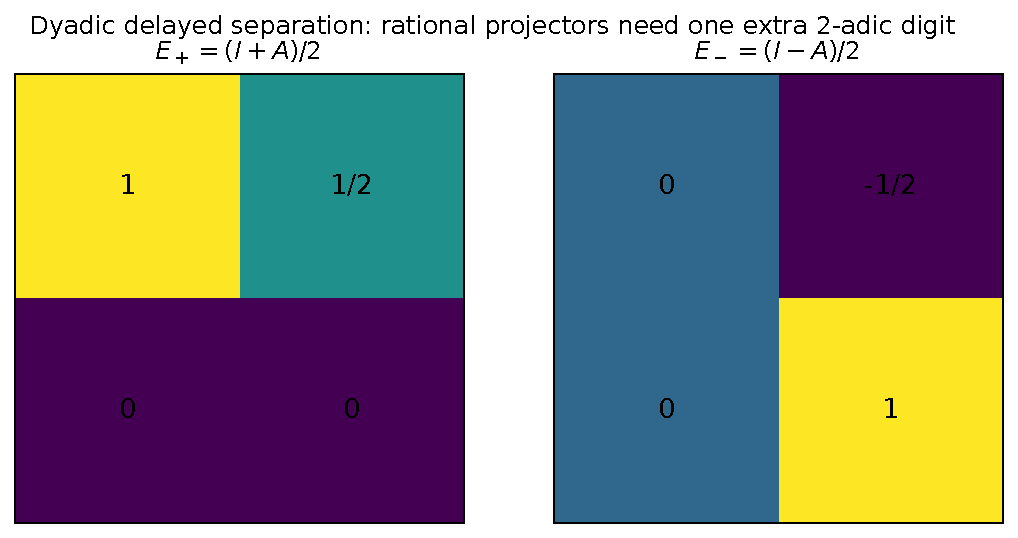
\includegraphics[width=0.88\textwidth]{07_dyadic_delayed_separation.pdf}
\caption{The rational sign projectors for an integral involution. Their denominator has $2$-adic weight one.}
\label{fig:dyadic-projectors}
\end{figure}

\begin{proposition}[Odd-adic versus dyadic behavior]\label{prop:dyadic-sign}
For every prime $p\ne2$, every entry of $E_+$ and $E_-$ is $p$-integral,
and each projector has exact local denominator weight zero. At $p=2$, each
projector has exact local denominator weight one; multiplication by $2$ makes
it integral, while the unscaled matrix is not integral:
\[
s_{2,\Z^2}(E_+)=s_{2,\Z^2}(E_-)=1.
\]
The characteristic factors $x-1$ and $x+1$ have resultant $2$. Its $2$-adic
valuation is one, exactly the two local projector weights above, and its
$p$-adic valuation is zero at every prime $p\ne2$.
\end{proposition}

\begin{proof}
The reduced denominators of the displayed entries are $1$ or $2$, which proves
the local integrality and minimality statements directly. The resultant is
\[
\Res(x-1,x+1)=2.
\]
Thus $v_2(2)=1$ and $v_p(2)=0$ for primes $p\ne2$.
\end{proof}

The two characteristic factors $x-1$ and $x+1$ have the same reduction in
$\F_2[x]$. The rational matrices $E_+$ and $E_-$ themselves cannot be reduced
modulo $2$, because their entries contain $1/2$. Consequently the integral
special fibre does not inherit their separate idempotent splitting, even
though the two projectors remain distinct over $\Q_2$. This is the simplest
model of delayed dyadic separation.

\begin{figure}[htbp]
\centering
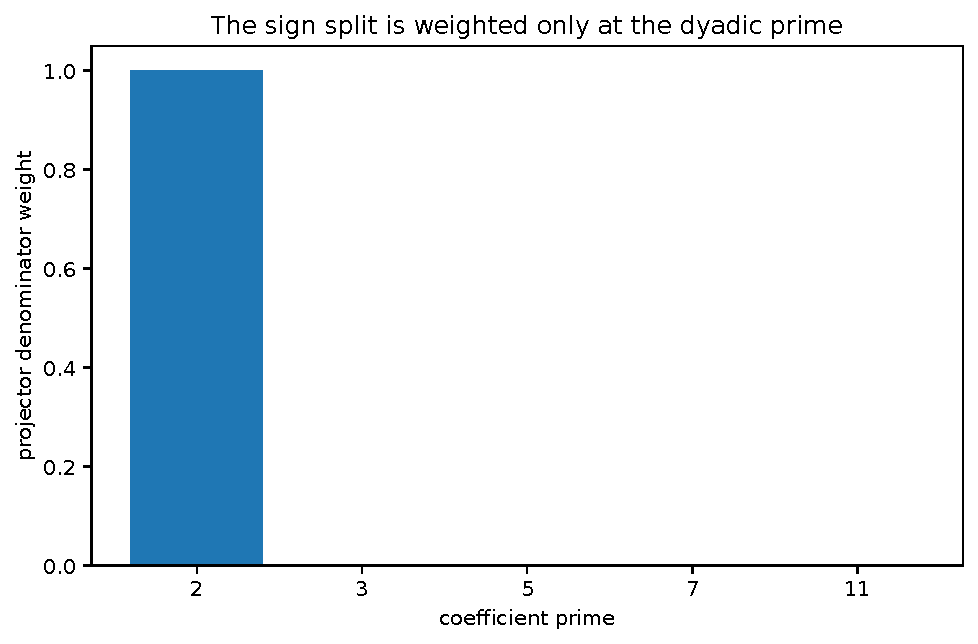
\includegraphics[width=0.84\textwidth]{08_odd_prime_separation.pdf}
\caption{The denominator weight of the sign projector is nonzero only at the prime two.}
\label{fig:odd-dyadic}
\end{figure}

\Needspace{7\baselineskip}
\subsubsection{Why coefficient packets remain available}

The failure of the character formula
\[
\frac12(I\pm A)
\]
to be integral does not invalidate coefficient selectors such as even and odd residue extraction. It shows that two distinct constructions must be distinguished:
\[
\boxed{
\text{integral address selector}
\quad\neq\quad
\text{character-average spectral projector}
}
\]
when the group order is not a unit. The first can remain exact over $\Z_2$; the second can acquire a denominator weight.


\section{Smith normal form and congruence lifting}\label{sec:smith}

The gluing module gives the exact common denominator of packet projectors.  Smith normal form gives the corresponding coordinate by coordinate solvability and branching rule.

\begin{standardfact}[Smith normal form over a discrete valuation ring]\label{fact:smith}
Let $M\in M_{m,n}(\OO)$.  There are invertible matrices
\[
U\in\operatorname{GL}_m(\OO),
\qquad
V\in\operatorname{GL}_n(\OO)
\]
such that
\[
UMV
=
\diag(\pi^{s_1},\ldots,\pi^{s_r},0,\ldots,0),
\]
where
\[
0\leq s_1\leq\cdots\leq s_r
\]
and $r$ is the rank over $K$.  The exponents are uniquely determined.  See \cite{Newman1972}.
\end{standardfact}

\begin{proposition}[Computing a packet weight from an inclusion matrix]\label{prop:weight_from_inclusion}
Choose an $\OO$ basis of $\Lambda$ and an $\OO$ basis of $\Lambda_{\mathrm{split}}$.  Let $B$ be the matrix of the inclusion
\[
\Lambda_{\mathrm{split}}\hookrightarrow\Lambda.
\]
If the Smith form of $B$ is
\[
\diag(\pi^{a_1},\ldots,\pi^{a_n}),
\qquad
0\leq a_1\leq\cdots\leq a_n,
\]
then
\[
G_{\Lambda,\Pcal}
\cong
\bigoplus_{j=1}^n\OO/\pi^{a_j}\OO,
\qquad
s_\Lambda(\Pcal)=\max\bigl(\{0\}\cup\{a_j:1\leq j\leq n\}\bigr).
\]
\end{proposition}

\begin{proof}
The gluing module is the cokernel of the inclusion matrix $B$.  Smith normal form gives its invariant factors.  The weight formula follows from \cref{thm:gluing_weight}.
\end{proof}

\begin{theorem}[Smith weighted congruence solve]\label{thm:smith_congruence}
Let $M\in M_{m,n}(\OO)$ have Smith exponents $s_1,\ldots,s_r$.  Let the residue field have size $q$, fix $L\geq1$, and consider
\[
Mx\equiv b\pmod{\pi^L}.
\]
Put
\[
\widetilde b=Ub
\]
for a Smith matrix $U$ as in \cref{fact:smith}.  The congruence is solvable if and only if
\[
\widetilde b_i\equiv0
\pmod{\pi^{\min(s_i,L)}}
\qquad(1\leq i\leq r)
\]
and
\[
\widetilde b_i\equiv0
\pmod{\pi^L}
\qquad(r<i\leq m).
\]
When it is solvable, the number of solutions in $(\OO/\pi^L\OO)^n$ is
\[
\boxed{
q^{(n-r)L+\sum_{i=1}^r\min(s_i,L)}.
}
\]
\end{theorem}

\begin{proof}
Set $x=Vy$.  Multiplying the congruence by $U$ reduces it to independent equations
\[
\pi^{s_i}y_i\equiv\widetilde b_i\pmod{\pi^L}
\qquad(1\leq i\leq r)
\]
and zero equations in the remaining rows.  Multiplication by $\pi^{s_i}$ on $\OO/\pi^L\OO$ has image equal to the elements divisible by $\pi^{\min(s_i,L)}$ and kernel of size
\[
q^{\min(s_i,L)}.
\]
Each of the $n-r$ unused variables is free and contributes $q^L$ choices.  Multiplying the independent counts gives the formula.
\end{proof}

\begin{corollary}[Obstruction and branching data]\label{cor:smith_obstruction}
The transformed entries of $\widetilde b$ that fail the stated divisibility conditions are the complete finite congruence obstructions.  When all obstructions vanish, the Smith exponents determine the number of solution branches at depth $L$.
\end{corollary}

\begin{proof}
This is exactly the solvability and counting statement of \cref{thm:smith_congruence} written in invariant coordinates.
\end{proof}

\begin{example}[Three weighted directions]\label{ex:smith_three}
Take $p=2$, $L=6$, and the diagonal weights
\[
(0,1,3).
\]
The right side
\[
(1,2,8)
\]
is admissible.  The three coordinate kernels have sizes
\[
1,
\quad2,
\quad8,
\]
so there are $16$ solutions.  Replacing the final entry $8$ by $4$ violates the required divisibility by $2^3$ and makes the system unsolvable.
\end{example}

\subsection{Concrete diagonal fibres over integer quotients}

Let $M$ be a matrix over a DVR. Smith normal form gives invertible matrices $U,V$ such that
\[
UMV
=
\diag(\pi^{s_1}u_1,\ldots,\pi^{s_r}u_r,0,\ldots,0),
\]
where each $u_i$ is a unit and
\[
0\le s_1\le\cdots\le s_r.
\]
The exponents $s_i$ are directional lifting weights.

\begin{theorem}[Concrete Smith-weighted congruence solve]\label{thm:smith-solve}
Let $p>1$ and consider the diagonal system over
$(\Z/(p^L)\Z)^d$
\[
\diag(p^{s_1},\ldots,p^{s_d})x=b
\pmod{p^L}.
\]
The system is solvable if and only if
\[
p^{\min(s_i,L)}\mid (b_i)_{\mathrm{val}}
\]
for every $i$, where $(b_i)_{\mathrm{val}}$ is the canonical natural
representative. Conditional on this admissibility condition, the number of
solutions is
\[
\boxed{
p^{\sum_{i=1}^d\min(s_i,L)}.
}
\]
If any coordinate is inadmissible, the solution set is empty and its
cardinality is zero.
\end{theorem}

\begin{proof}
Lean proves the one-coordinate arithmetic directly over
$\mathbb Z/p^L\mathbb Z$ for every $p>1$:
\[
\bigl(\exists x\in\mathbb Z/p^L\mathbb Z:\quad p^s x=b\pmod{p^L}\bigr)
\quad\Longleftrightarrow\quad
p^{\min(s,L)}\mid b_{\mathrm{val}},
\]
where $b_{\mathrm{val}}$ is the canonical natural representative, and every
admissible fibre has exactly $p^{\min(s,L)}$ elements. The coordinates are
independent, so the product equivalence gives the displayed global count. If
one coordinate fibre is empty, the global fibre is empty. Lean proves both the
global solvability equivalence and the conditional count, including
cardinality zero on the inadmissible branch.
\end{proof}

For an arbitrary DVR $\OO$ with residue-field cardinality $q$, the analogous
formula
\[
q^{\sum_i\min(s_i,L)}
\]
is a classical consequence of the corresponding one-coordinate solvability
and fibre-cardinality facts. In the Lean development this general form is
\emph{certificate-explicit}: those coordinate facts may be supplied to the
abstract product API, but they are not derived from a formalized general-DVR
structure theorem. Construction and diagonalization of Smith normal form for
an arbitrary DVR matrix also remain classical input; see
\cite{Serre1979,Lang2002}.

If a Smith form is rank deficient, a literal zero diagonal factor requires
the corresponding target coordinate to vanish modulo $p^L$ and then
contributes all $p^L$ possible coordinate values. In the concrete quotient it
can equivalently be represented by any weight $s_i\ge L$, since
$p^{s_i}=0$ in $\Z/(p^L)\Z$; the theorem then gives exactly that condition and
factor. The numbered theorem begins after the diagonal data have been
supplied and does not construct the Smith form.

\begin{example}
At $p=2$, depth $L=6$, and weights $(0,1,3)$, the right-hand side $(1,2,8)$ is admissible. The coordinate kernels have sizes
\[
1,2,8,
\]
so the system has $16$ solutions. Replacing $8$ by $4$ in the final coordinate violates the divisibility condition and makes the system unsolvable.
\end{example}

This theorem is the multivariable version of precision delay. A coordinate with weight $s_i$ contributes both a solvability threshold and $s_i$ units of branching until the ambient depth truncates it.


\section{Linear refinement defects}\label{sec:defects}

Exact coordinate refinement concerns two representations of the same object.  In applications one often chooses a new coarse operator rather than conjugating the fine operator exactly.  The difference is measured by an intertwining defect.

Let $X_f$ and $X_c$ be vector spaces or Banach spaces over a common field, and let
\[
C:X_f\longrightarrow X_c
\]
be a linear map,
and let
\[
T_f\in\End(X_f),
\qquad
T_c\in\End(X_c).
\]
Define
\[
\Delta=CT_f-T_cC.
\]

\begin{theorem}[Power defect identity]\label{thm:power_defect}\label{thm:power-defect}
For every integer $n\geq1$,
\[
CT_f^n-T_c^nC
=
\sum_{k=0}^{n-1}T_c^{n-1-k}\Delta T_f^k.
\]
\end{theorem}

\begin{proof}
The statement is clear for $n=1$.  For the induction step, write
\[
CT_f^{n+1}-T_c^{n+1}C
=
(CT_f^n-T_c^nC)T_f+T_c^n(CT_f-T_cC)
\]
and apply the induction hypothesis.
\end{proof}

\begin{corollary}[Power norm bound]\label{cor:power_norm}
For bounded operators between Banach spaces,
\[
\|CT_f^n-T_c^nC\|
\leq
\|\Delta\|
\sum_{k=0}^{n-1}
\|T_c\|^{n-1-k}\|T_f\|^k.
\]
\end{corollary}

\begin{proof}
Apply the triangle inequality and submultiplicativity to \cref{thm:power_defect}.
\end{proof}

\begin{corollary}[Norm bound]\label{cor:defect-norm}
For a submultiplicative operator norm,
\[
\|CT_f^n-T_c^nC\|
\le
\|\Delta\|
\sum_{k=0}^{n-1}
\|T_c\|^{n-1-k}\|T_f\|^k.
\]
If $\|T_f\|,\|T_c\|\le\rho$, then
\[
\boxed{
\|CT_f^n-T_c^nC\|
\le n\rho^{n-1}\|\Delta\|.
}
\]
\end{corollary}

\begin{corollary}[Polynomial defect]\label{cor:polynomial_defect}
For
\[
p(z)=\sum_{n=0}^Na_nz^n,
\]
we have
\[
Cp(T_f)-p(T_c)C
=
\sum_{n=1}^Na_n
\sum_{k=0}^{n-1}T_c^{n-1-k}\Delta T_f^k.
\]
\end{corollary}

\begin{proof}
The constant terms cancel because $CI=IC$.  Apply \cref{thm:power_defect} to every positive power and sum.
\end{proof}

\begin{theorem}[Resolvent defect identity]\label{thm:resolvent_defect}\label{thm:resolvent-defect}
If $z-T_f$ and $z-T_c$ are invertible, then
\[
C(z-T_f)^{-1}-(z-T_c)^{-1}C
=
(z-T_c)^{-1}\Delta(z-T_f)^{-1}.
\]
\end{theorem}

\begin{proof}
Multiply the claimed identity on the left by $z-T_c$ and on the right by $z-T_f$.  The left side becomes
\[
(z-T_c)C-C(z-T_f)
=
CT_f-T_cC
=
\Delta.
\]
Multiplying back by the two resolvents proves the formula.
\end{proof}

\subsection{One-sided inverse witnesses and operator-norm control}
For continuous linear maps, the same identity gives the certified norm bound
\[
\boxed{
\|C R_f-R_c C\|
\le \|R_c\|\,\|\Delta\|\,\|R_f\|,
}
\]
from a left inverse witness for the coarse scalar shift and a right inverse
witness for the fine scalar shift. These one-sided witnesses are sufficient
for the displayed identity, although they need not by themselves define
two-sided resolvents. If $\Delta=0$, Lean also proves, for every finite
polynomial $p$, the exact compatibility
\[
\boxed{C\,p(T_f)=p(T_c)\,C,}
\]
in both the algebraic and continuous-linear-map settings. Thus all powers,
polynomial actions, and the explicitly witnessed resolvents intertwine with
coarse reconstruction. This is the linear prototype of the more general
refinement-defect theory reserved for Paper III.

\begin{figure}[htbp]
\centering
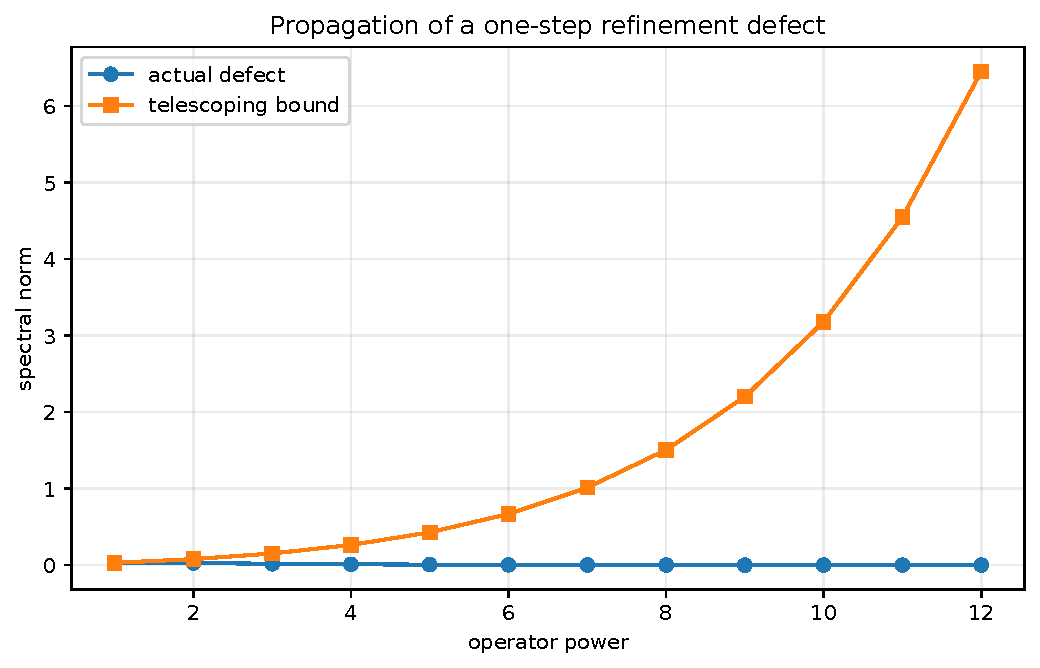
\includegraphics[width=0.88\textwidth]{09_refinement_defect_bound.pdf}
\caption{A controlled one-step defect and its telescoping norm bound under repeated operator application.}
\label{fig:defect-bound}
\end{figure}


\subsection{Analytic functional calculus}
\begin{theorem}[Holomorphic functional calculus defect]\label{thm:holomorphic_defect}
Let $X_f$ and $X_c$ be complex Banach spaces, and let $C:X_f\to X_c$, $T_f$, and $T_c$ be bounded complex-linear maps.  Let $h$ be holomorphic on an open set $U$ containing both spectra.  Let $\Gamma$ be an admissible finite rectifiable Cauchy cycle in $U$ and in both resolvent sets, with winding number one on the union of the spectra and zero outside $U$.  The length of a cycle counts multiplicities.  Then
\[
Ch(T_f)-h(T_c)C
=
\frac{1}{2\pi i}
\int_\Gamma
h(z)(z-T_c)^{-1}\Delta(z-T_f)^{-1}\,dz.
\]
Consequently,
\begin{align*}
\|Ch(T_f)-h(T_c)C\|
&\leq
\frac{\operatorname{length}(\Gamma)}{2\pi}
\sup_{z\in\Gamma}|h(z)|\,\|\Delta\|\\
&\quad\times
\sup_{z\in\Gamma}\|(z-T_c)^{-1}\|
\sup_{z\in\Gamma}\|(z-T_f)^{-1}\|.
\end{align*}
\end{theorem}

\begin{proof}
The holomorphic functional calculus gives
\[
h(T)
=
\frac{1}{2\pi i}
\int_\Gamma h(z)(z-T)^{-1}\,dz.
\]
Subtract the two formulas after composing with $C$, then use \cref{thm:resolvent_defect} inside the integral.  The norm estimate follows from the standard contour bound.
\end{proof}

\begin{theorem}[Exponential defect identity]\label{thm:exponential_defect}
Let $C:X_f\to X_c$, $T_f$, and $T_c$ be bounded linear maps between Banach spaces over a common field.  For real $t$, use real or complex spaces; for complex $t$, use complex spaces and complex-linear maps.  Then
\[
Ce^{tT_f}-e^{tT_c}C
=
\int_0^t e^{(t-s)T_c}\Delta e^{sT_f}\,ds,
\]
where the integral is taken along the straight segment from $0$ to $t$ when $t$ is complex.  For real $t\geq0$,
\[
\|Ce^{tT_f}-e^{tT_c}C\|
\leq
\|\Delta\|
\int_0^t
\|e^{(t-s)T_c}\|
\|e^{sT_f}\|\,ds.
\]
\end{theorem}

\begin{proof}
For real $t$, differentiate
\[
F(s)=e^{(t-s)T_c}Ce^{sT_f}.
\]
We obtain
\[
F'(s)=e^{(t-s)T_c}\Delta e^{sT_f}.
\]
Integration from $0$ to $t$ gives the identity.  The complex statement follows by the same calculation along the straight segment.  The norm bound follows from the integral formula.
\end{proof}

\subsection{Several refinement levels}

Let
\[
C_\ell:X_{\ell+1}\longrightarrow X_\ell
\]
be linear maps for $0\leq\ell<L$, and let $T_\ell\in\End(X_\ell)$.  Put
\[
\Delta_\ell=C_\ell T_{\ell+1}-T_\ell C_\ell.
\]
For $a<b$, write
\[
C_{a,b}=C_aC_{a+1}\cdots C_{b-1},
\]
with $C_{a,a}=I$.

\begin{theorem}[Multilevel defect decomposition]\label{thm:multilevel_defect}
The total defect from level $L$ to level zero is
\[
C_{0,L}T_L-T_0C_{0,L}
=
\sum_{\ell=0}^{L-1}
C_{0,\ell}\Delta_\ell C_{\ell+1,L}.
\]
For bounded maps,
\[
\|C_{0,L}T_L-T_0C_{0,L}\|
\leq
\sum_{\ell=0}^{L-1}
\|C_{0,\ell}\|
\|\Delta_\ell\|
\|C_{\ell+1,L}\|.
\]
\end{theorem}

\begin{proof}
Insert the intermediate terms
\[
C_{0,\ell}T_\ell C_{\ell,L}
\]
for $0\leq\ell\leq L$.  Consecutive differences telescope.  The difference between the terms indexed by $\ell+1$ and $\ell$ is
\[
C_{0,\ell}(C_\ell T_{\ell+1}-T_\ell C_\ell)C_{\ell+1,L}.
\]
Summing gives the identity.  The norm estimate follows from the triangle inequality.
\end{proof}

\begin{example}[A visible one step defect]\label{ex:defect_example}
Let $X_f=\bbk^2$, let $X_c=\bbk$, and let
\[
C(x_1,x_2)=x_1.
\]
Take
\[
T_f=
\begin{pmatrix}
a&b\\
c&d
\end{pmatrix},
\qquad
T_c=(a).
\]
Then
\[
\Delta=CT_f-T_cC=(0,b).
\]
The coarse operator is exactly compatible with the fine operator precisely when the discarded coordinate does not feed into the retained coordinate.  The entry $c$ does not appear in the one step defect because it moves information in the opposite direction.  It can still affect later powers through the terms in \cref{thm:power_defect}.
\end{example}

\begin{corollary}[Exact compatibility]\label{cor:exact_compatibility}
If every one step defect $\Delta_\ell$ vanishes, then
\[
C_{0,L}p(T_L)=p(T_0)C_{0,L}
\]
for every polynomial $p$.  The analogous resolvent, holomorphic, and exponential identities also hold whenever the relevant expressions are defined.
\end{corollary}

\begin{proof}
The total one step defect vanishes by \cref{thm:multilevel_defect}.  Apply \cref{cor:polynomial_defect,thm:resolvent_defect,thm:holomorphic_defect,thm:exponential_defect}.
\end{proof}

\section{Worked realizations in the common operator language}

\subsection{Signal polyphase coordinates}

Let $x=(x_n)_{n\in\Z}\in c_{00}(\Z;R)$ and let the seed be $\delta_0$
under the bilateral shifts $(S^r\delta_0)_n=\delta_{n,r}$. This makes the
algebraic span and every displayed sum finite. The $N$ packets are
\[
x_j[m]=x[Nm+j].
\]
Synthesis interleaves these sequences. A finite-impulse-response linear
time-invariant filter becomes an $N\times N$ matrix of transfer blocks.
Refining from $N$ to $M$ with $N\mid M$ splits each coarse phase into its
descendants without changing the reconstructed signal. The same formulas
extend to standard sequence completions when the synthesis series converges;
this is the usual polyphase viewpoint from multirate filter banks
\cite{Vaidyanathan1993}.

\subsection{Transfer-block sparsity}

A banded operator need not remain banded after residue reordering, but its
nonzero couplings become a structured packet graph. With the convention
$(S_rx)_n=x_{n-r}$, the only active transfer is
\[
P_{N,j+r}S_rP_{N,j},
\]
with indices taken modulo $N$. More general finite stencils produce a finite set of active phase differences.

\begin{figure}[htbp]
\centering
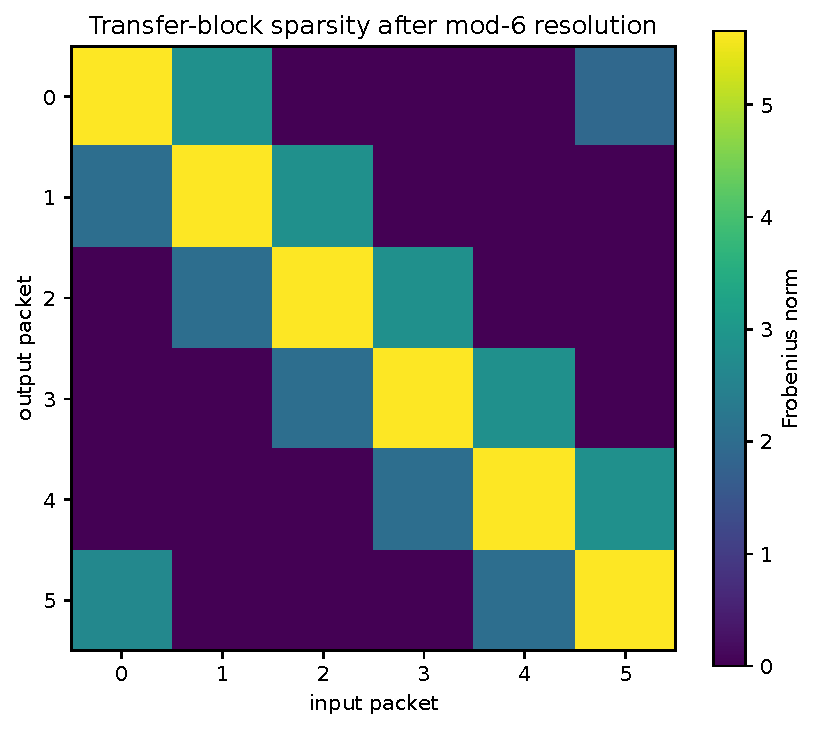
\includegraphics[width=0.76\textwidth]{10_transfer_block_sparsity.pdf}
\caption{Packet-block norms for a finite stencil. The original operator is exactly reconstructed from a sparse transfer pattern.}
\label{fig:block-sparsity}
\end{figure}

\subsection{A short Smith-coordinate realization}\label{sec:smith-realization}

Normalize an impedance by $z=Z/Z_0$ and write
\[
\Gamma=\frac{z-1}{z+1}.
\]
A phase action on the reflection disk is
\[
\Gamma\mapsto\omega_N^k\Gamma.
\]
Pulling it back gives
\[
T_{N,k}(z)
=
\frac{(1+\omega_N^k)z+(1-\omega_N^k)}
{(1-\omega_N^k)z+(1+\omega_N^k)}.
\]
For $N=2$ and $k=1$,
\[
T_{2,1}(z)=\frac1z,
\qquad z\ne0,-1.
\label{eq:smith-inversion}
\]
Thus the nontrivial first-level phase action exchanges normalized impedance
and admittance. Calling these values ``packets'' is geometric terminology for
the sampled orbit, not an assertion that the two values form linear
idempotent ranges. Higher $2$-power refinements sample the same reflection
circle at progressively finer electrical phases; compare the standard Smith
chart conventions in \cite{pozar2012}.

\begin{figure}[htbp]
\centering
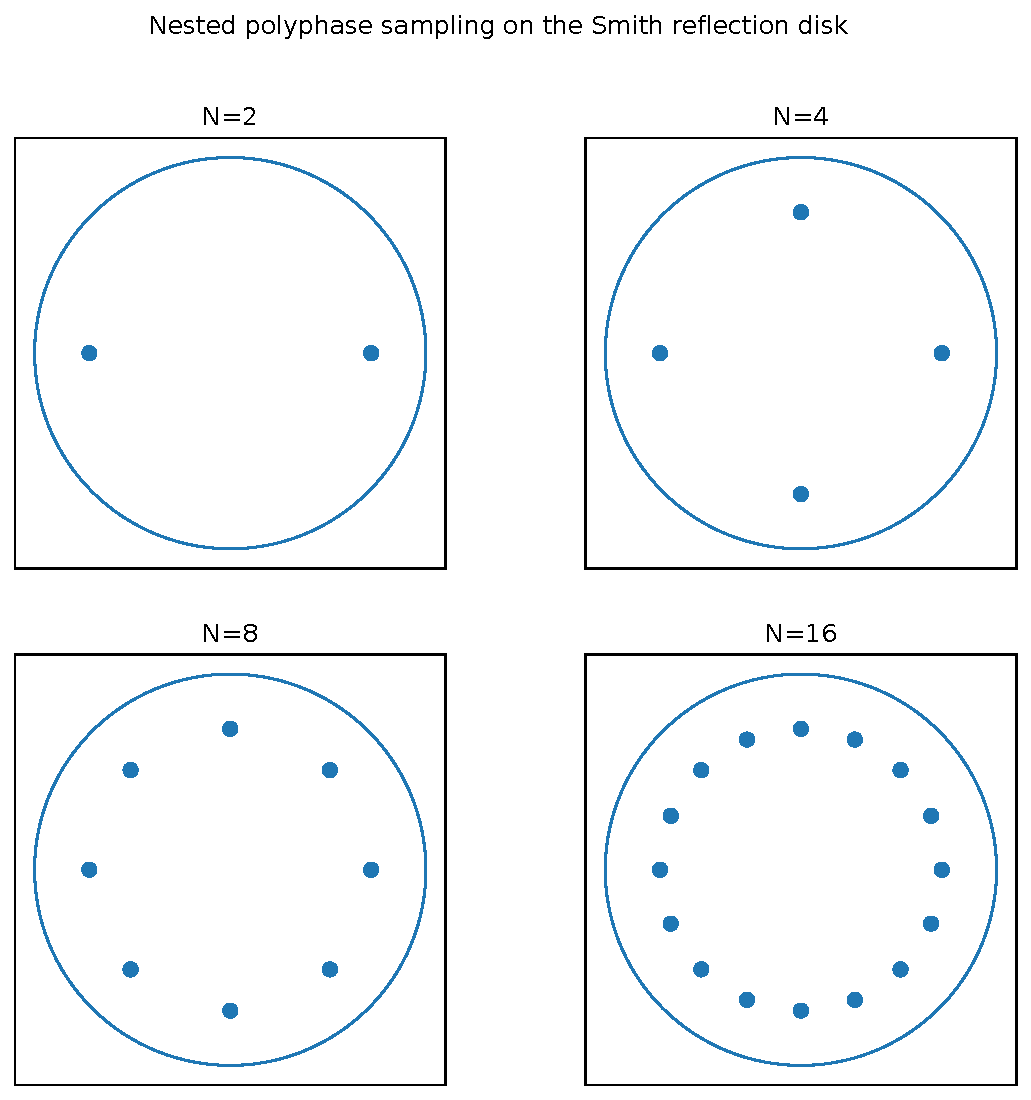
\includegraphics[width=0.88\textwidth]{11_smith_polyphase_orbit.pdf}
\caption{Nested $2$-power phase orbits on the Smith reflection disk. The full Smith-chart treatment is deferred to the signal paper.}
\label{fig:smith-orbit}
\end{figure}

The symmetric weight
\[
w_{\mathrm{Smith}}(\Gamma)
=
\frac1{|1-\Gamma|^2}
+
\frac1{|1+\Gamma|^2}
\]
indicates where small reflection-coordinate errors produce large impedance or admittance errors.

\begin{figure}[htbp]
\centering
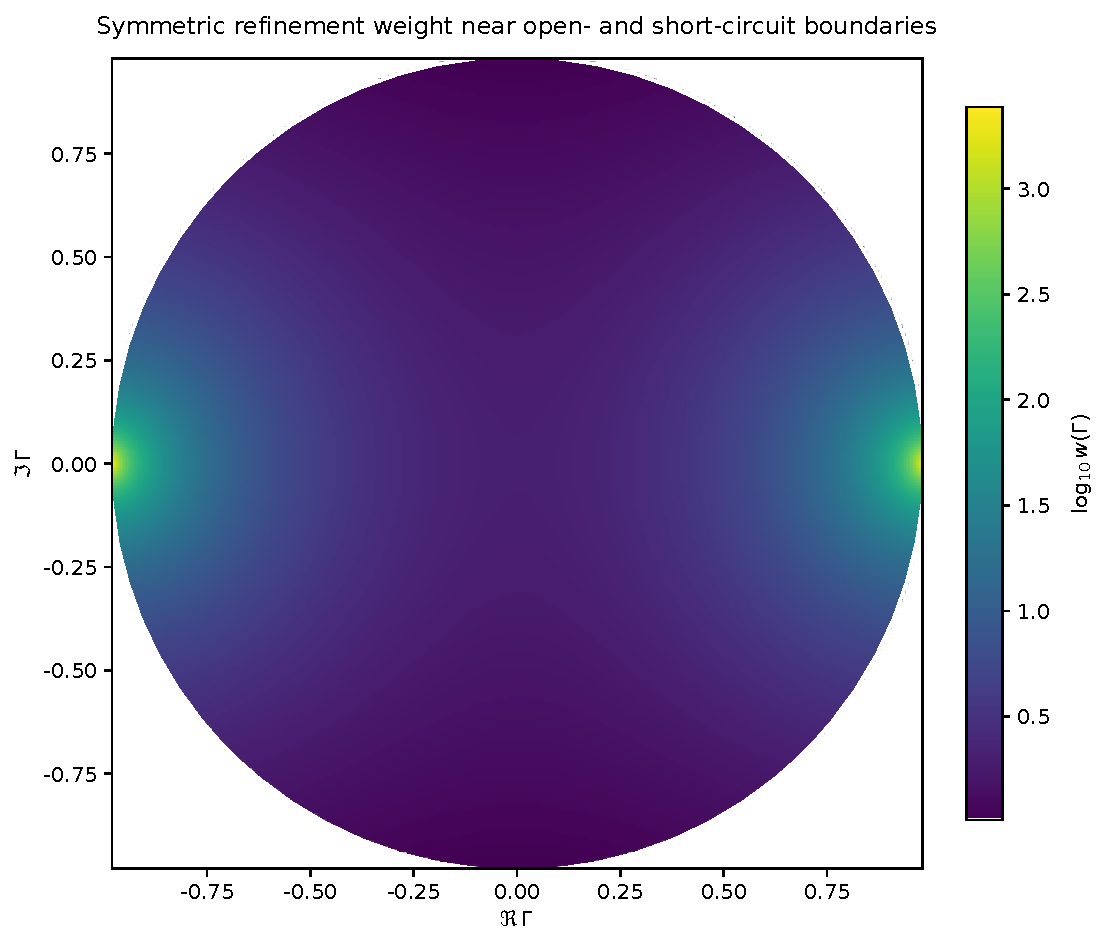
\includegraphics[width=0.70\textwidth]{12_smith_adaptive_weight.pdf}
\caption{A symmetric refinement weight concentrated near the open- and short-circuit boundary points.}
\label{fig:smith-weight}
\end{figure}


\section{Finite computational certificates}
The following results and tables are the recorded v1.2.1 finite implementation evidence.  They do not certify the expanded lattice or analytic statements in Lean.  Current reproduction outcomes are reported in the verification files accompanying this edition.


All numerical work in this paper is finite and reproducible. It tests the
Python implementation of identities proved or certificate-checked above; it
does not replace those arguments or the Lean kernel checks. Release 1.2.1 runs
forty-eight tests, including invalid-input contracts, refinement transitivity,
transfer-block aggregation, Fourier/DFT agreement, brute-force Smith fibre
counts, and consistency of the stored JSON and CSV records.

\begin{table}[htbp]
\centering
\caption{Representative numerical and symbolic checks.}
\begin{tabularx}{\textwidth}{L{0.54\textwidth}Y}
\toprule
Check & Result \\
\midrule
Packet synthesis residuals for moduli $2,3,4,6,8,12$ & $0$ \\
Nested refinement residuals for $2\to4$, $2\to8$, $3\to6$, $3\to12$, $4\to8$, $4\to12$, $6\to12$ & $0$ \\
Dyadic--odd CRT residuals for $4\times3$, $8\times3$, $4\times5$, $8\times5$ & $0$ \\
Maximum finite-Fourier projector residual & $6.60\times10^{-15}$ \\
Weighted inverse residual modulo $2^{10}$ & $0$ \\
Weighted inverse residual modulo $3^8$ & $0$ \\
Weighted inverse residual modulo $5^7$ & $0$ \\
Difference between filtered and direct modular inverses & $0$ \\
Transfer-zeta coefficients versus direct walk enumeration through weight $30$ & exact match \\
Dyadic sign-projector resultant weight & $v_2(2)=1$ \\
Odd-prime sign-projector resultant weight at $3$ & $v_3(2)=0$ \\
Power-defect telescoping identity residual & at most $6.94\times10^{-18}$ \\
Resolvent-defect identity residual & $1.09\times10^{-17}$ \\
Smith $N=2$ phase versus $z\mapsto1/z$ & residual below $1.4\times10^{-16}$ \\
\bottomrule
\end{tabularx}
\end{table}

\begin{certificate}[Weighted inverse]
For the tested diagonal-plus-transfer matrices, the filtered inverse agrees exactly with direct modular inversion at all tested precisions:
\[
2^{10},\qquad3^8,\qquad5^7.
\]
The maximum modular residual is zero in every case.
\end{certificate}

\begin{certificate}[Transfer zeta]
The rational function
\[
\frac{-t^3}{t^9-t^7-t^6-t^5+2t^4+t^3+t^2-1}
\]
was expanded through degree $30$. Every coefficient agrees with direct weighted-walk enumeration.
\end{certificate}

\begin{certificate}[Dyadic separation]
The code verifies exactly that the two rational sign projectors are idempotent, orthogonal, and complementary, that scaling by $2$ makes both integral, and that the same projectors are already integral modulo every tested odd prime.
\end{certificate}


\section{Scope and limits}\label{sec:limits}

The exact statements above have several deliberate boundaries.

First, refinement is a change of coordinates, not a truncation theorem.  If a numerical method discards fine packets, the resulting error must be estimated separately.

Second, the weighted inverse is linear.  A nonlinear map creates higher order interactions among packet coordinates.  Those interactions are not contained in the path formula of \cref{thm:weighted_inverse}.

Third, a resultant is only a denominator bound.  The exact weight depends on the lattice and is given by \cref{thm:gluing_weight}.  The two examples in \cref{ex:loose_resultant,ex:lattice_dependence} show that the same eigenvalue separation can give different integral packet weights.

Fourth, the dyadic sign example is a model rather than a classification of all phenomena at the prime two.  Character averages, trace splittings, quadratic refinements, and deformation projectors must each be checked on their own lattices.

Finally, the defect formulas do not prove that a chosen coarse operator is a good approximation.  They say exactly how a known one step defect propagates.  A useful approximation theorem must also bound that defect in the problem under study.



\appendix
\section{Notation table}

\begin{longtable}{L{0.28\textwidth}L{0.64\textwidth}}
\toprule
Symbol & Meaning \\
\midrule
\endhead
$P_{\ell,\alpha}$ & packet projector at refinement level $\ell$ \\
$I_\ell$ & packet address set at level $\ell$ \\
$\beta\succ\alpha$ & fine packet $\beta$ is a child of coarse packet $\alpha$ \\
$\cA_\ell,\cS_\ell$ & packet analysis and synthesis maps \\
$J_{\ell+1,\ell}$ & exact coordinate refinement map \\
$C_{\ell,\ell+1}$ & exact fine-to-coarse coordinate regrouping \\
$T^{(\ell)}_{\beta\alpha}$ & transfer block $P_{\ell,\beta}TP_{\ell,\alpha}$ \\
$P_{N,j}$ & residue or phase selector for address $j\pmod N$ \\
$w(e)$ & positive filtration weight of a transfer edge \\
$W(\gamma)$ & cumulative weight of a transfer word or graph walk \\
$A(t)$ & polynomial weighted adjacency matrix \\
$Z_{s,t}(t)$ & weighted transfer-zeta function from vertex $s$ to vertex $t$ \\
$s_{\pi,\Lambda}(E)$ & lattice-dependent separation weight of a rational projector, when a clearing exponent exists \\
$\Delta$ & one-step linear refinement defect $CT_f-T_cC$ \\
\bottomrule
\end{longtable}

\section{Algorithmic forms}\label{sec:algorithms}

\subsection{Residue analysis and synthesis}\label{alg:residue}

\begin{lstlisting}
def analyze_residues(x, N):
    require N > 0
    return [x[j::N] for j in range(N)]

def synthesize_residues(packets):
    N = len(packets)
    require packet lengths fit one N-way interleaving
    y = empty(sum(len(p) for p in packets))
    for j, packet in enumerate(packets):
        y[j::N] = packet
    return y
\end{lstlisting}

The verified contract is
$\operatorname{synthesize}(\operatorname{analyze}(x,N))=x$. The Lean
counterpart uses range-restricted packet coordinates and proves both inverse
laws, while the finite Python routine checks the concrete array realization.

\subsection{Weighted finite-precision inverse}\label{alg:weighted-inverse}

\begin{lstlisting}
Dinv = inverse(D)                       # certified on both sides
edge[e] = Dinv @ H_edge[e]
require Dinv @ H == sum(edge[e] for e in edges)
require edge[e] lies in filtration[weight[e]]
m = certified_lower_bound(weight)       # 1 <= m <= weight[e]
N = (L + m - 1) // m                    # so L <= m*N
S = 0
for n in range(N):
    for word in edge_tuples(edges, n):
        if sum(weight[e] for e in word) < L:
            S += (-1)**n * ordered_product(edge[e] for e in word)
return q_L(S @ Dinv)
\end{lstlisting}

Lean proves that the mapped pruned sum is exactly the mapped finite geometric
inverse. The lower bound $m$ gives $m|\gamma|\le W(\gamma)$, so
$L\le mN$ derives $q_L(A^N)=0$ from the filtration certificate and makes the
returned value a two-sided inverse of $q_L(D+H)$. The Lean lemma
$L\le m\lceil L/m\rceil$ justifies the displayed executable cutoff for
$m>0$. Taking $m=1$ and $N=L$ gives
the unconditional positive-weight cutoff. The Python implementation checks the
DVR matrix specialization against direct modular inversion.

\subsection{Transfer-zeta walk construction}\label{alg:path-zeta}

\begin{lstlisting}
def coefficient(G, start, target, n):
    total = 0
    for length in range(n + 1):
        for word in edge_tuples(G, length):
            if is_walk(word, start, target) and weight(word) == n:
                total += 1
    return total

A[i,j] = sum(t**weight(e) for distinct edges e from i to j)
T = I - A
Q = det(T)
H = adjugate(T)
P = H[start, target]
assert Q.coeff(0) == 1
Z = coefficient_series(G, start, target)
prove Q * Z == P
\end{lstlisting}

Positive weights make the coefficient loop finite because every contributing
word has length at most $n$. Lean proves the enumeration correct, derives its
first-edge recurrence, proves $(I-A)Z=I$, constructs the determinant/adjugate
inverse, and identifies the two matrices by inverse uniqueness. Thus the
normalized $QZ=P$ identity and its induced recurrence follow from finite graph
data. The Python companion repeats the exact symbolic construction as an
executable cross-check; it is not an oracle used by the Lean proof.

\section{Proof dependency map}

\begin{figure}[htbp]
\centering
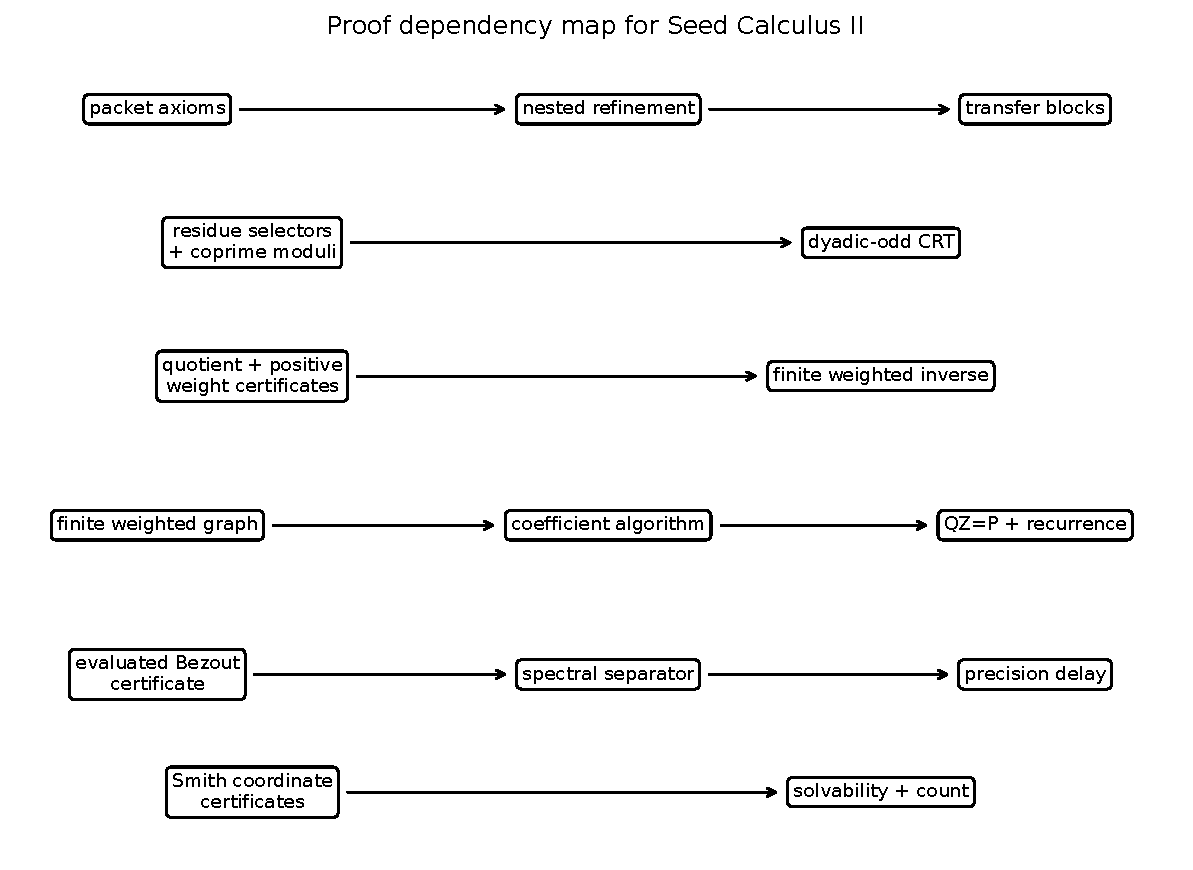
\includegraphics[width=0.96\textwidth]{13_theorem_dependency.pdf}
\caption{The dependency structure of Paper II. Coordinate coherence, residue/CRT, weighted inversion, automatic finite-graph transfer rationality, and integral separation are distinct branches with explicit inputs.}
\label{fig:dependency}
\end{figure}

The proof order is:
\[
\begin{aligned}
&\text{complete packet axioms}
  \Rightarrow\text{finite-packet uniqueness and coordinate coherence}\\
&\qquad\Rightarrow\text{coordinate naturality and refined transfer blocks},\\
&\text{residue selectors and a finite Fourier table}
  \Rightarrow\text{Fourier formulas},\\
&\text{coprime moduli}\Rightarrow\text{dyadic--odd formulas},\\
&\text{quotient, filtration, and edge-weight certificates}
  \Rightarrow\text{explicit pruned inverse},\\
&\text{finite positive-weight graph}
  \Rightarrow\text{semantic enumeration and first-edge recurrence}\\
&\qquad\Rightarrow\det/\operatorname{adj}\text{ rationality and recurrence},\\
&\text{minimal evaluated B\'ezout data and inverse-unit lattice action}\\
&\qquad\Rightarrow\text{separation bound, upward closure, and precision delay},\\
&\text{concrete }\mathbb Z/p^L\mathbb Z\text{ coordinate fibres}
  \Rightarrow\text{finite Smith product count},\\
&\text{one-step typed defect}
  \Rightarrow\text{powers, polynomial actions, and witnessed resolvents}.
\end{aligned}
\]

The transfer-zeta walk branch is logically independent of operator inversion. Its
rationality conclusion now follows from finite graph data, rather than from a
supplied $QZ=P$ premise. Likewise, CRT factorization follows directly from
residue selectors and coprimality; it does not require the abstract refinement
theorem, although it supplies a concrete refinement family. General Smith
diagonalization and construction of polynomial B\'ezout/resultant data remain
inputs upstream of the formalized post-certificate branches.

\section{Edition and proof scope}\label{sec:edition-scope}
The traditional article is a single topic-ordered edition.  The expanded ordinary-proof branch supplies the main narrative, including common refinements, complete filtered inversion, exact lattice gluing, rectangular Smith congruences, and analytic and multilevel defects.  The canonical v1.2.1 release supplies the explicitly certified specializations, finite graph construction, worked realizations, and three algorithm specifications.

The frozen Lean contract has 25 rows: 21 canonical numbered items, one Smith-phase identity, and three algorithm specifications.  A shared human theorem can serve more than one source address, and a contract row may use several Lean declarations.  These are distinct counting units.  In particular, the complete inverse-limit filtered theorem, general lattice gluing theorem, holomorphic and exponential calculus, and multilevel statements are ordinary written proofs here; the inherited 25-row contract does not automatically cover them.

The source statements have received only the recorded local hypothesis and endpoint repairs.  The original branch sources are preserved beside this editable edition.  The source crosswalk records original labels, final labels, display numbers, pages, and the relationship between the scopes.  The proof-preservation audit compares every inherited proof body.  No fresh Lean compiler replay is asserted by this article.

The standalone visual guide gives exact worked models.  The Lean guide explains declaration-level contracts, pins, and recorded build evidence.  Illustrations and finite tests support understanding and implementation checks; they do not replace universal proofs.
\bibliographystyle{plain}\bibliography{references}
\end{document}
